\ifx\wholebook\relax \else
% ------------------------

\documentclass[UTF8]{article}
%------------------- Other types of document example ------------------------
%
%\documentclass[twocolumn]{IEEEtran-new}
%\documentclass[12pt,twoside,draft]{IEEEtran}
%\documentstyle[9pt,twocolumn,technote,twoside]{IEEEtran}
%
%-----------------------------------------------------------------------------
%
% loading packages
%

\RequirePackage{ifpdf}
\RequirePackage{ifxetex}

%
%
\ifpdf
  \RequirePackage[pdftex,%
       bookmarksnumbered,%
              colorlinks,%
          linkcolor=blue,%
              hyperindex,%
        plainpages=false,%
       pdfstartview=FitH]{hyperref}
\else\ifxetex
  \RequirePackage[bookmarksnumbered,%
               colorlinks,%
           linkcolor=blue,%
               hyperindex,%
         plainpages=false,%
        pdfstartview=FitH]{hyperref}
\else
  \RequirePackage[dvipdfm,%
        bookmarksnumbered,%
               colorlinks,%
           linkcolor=blue,%
               hyperindex,%
         plainpages=false,%
        pdfstartview=FitH]{hyperref}
\fi\fi
%\usepackage{hyperref}

% other packages
%--------------------------------------------------------------------------
\usepackage{graphicx, color}
\usepackage{subfig}
\usepackage{multicol}
\usepackage{tikz}
\usetikzlibrary{matrix,positioning,shapes}

\usepackage{amsmath, amsthm, amssymb} % for math
\usepackage{exercise} % for exercise
\usepackage{import} % for nested input

%
% for programming
%
\usepackage{verbatim}
\usepackage{fancyvrb}
\usepackage{listings}
%\usepackage{algorithmic} %old version; we can use algorithmicx instead
%\usepackage[plain]{algorithm} %remove rule (horizontal line on top/below the algorithm
\usepackage{algorithm} %to remove rules change to \usepackage[plain]{algorithm}
%\usepackage{algorithm2e}
\usepackage[noend]{algpseudocode} %for pseudo code, include algorithmicsx automatically
\usepackage{appendix}
\usepackage{makeidx} % for index support
\usepackage{titlesec}

\usepackage[cm-default]{fontspec}
\usepackage{xunicode}
%\usepackage{fontenc}
\usepackage{textcomp}
\usepackage{url}

% detect and select Chinese font
% ------------------------------
% the following cmd can list all availabe Chinese fonts in host.
% fc-list :lang=zh
\def\myfont{STSong}  % Under Mac OS X
\def\linuxfallback{WenQuanYi Micro Hei} % Under Linux
\def\winfallback{SimSun} % Under Windows
\suppressfontnotfounderror1 % Avoid setting exit code (error level) to break make process
\count255=\interactionmode
\batchmode
\font\foo="\myfont"\space at 10pt
\ifx\foo\nullfont
  \font\foo = "\linuxfallback"\space at 10pt
  \ifx\foo\nullfont
    \font\foo = "\winfallback"\space at 10pt
    \ifx\foo\nullfont
      \errorstopmode
      \errmessage{no suitable Chinese font found}
    \else
      \let\myfont=\winfallback % Windows
    \fi
  \else
    \let\myfont=\linuxfallback % Linux
  \fi
\fi
\interactionmode=\count255
\setmainfont[Mapping=tex-text]{\myfont}
\setmonofont[Scale=MatchLowercase]{Monaco}   % 英文等宽字体

\XeTeXlinebreaklocale "zh"  % to solve the line breaking issue
\XeTeXlinebreakskip = 0pt plus 1pt minus 0.1pt

\titleformat{\paragraph}
{\normalfont\normalsize\bfseries}{\theparagraph}{1em}{}
\titlespacing*{\paragraph}
{0pt}{3.25ex plus 1ex minus .2ex}{1.5ex plus .2ex}

\lstdefinelanguage{Smalltalk}{
  morekeywords={self,super,true,false,nil,thisContext}, % This is overkill
  morestring=[d]',
  morecomment=[s]{"}{"},
  alsoletter={\#:},
  escapechar={!},
  literate=
    {BANG}{!}1
    {UNDERSCORE}{\_}1
    {\\st}{Smalltalk}9 % convenience -- in case \st occurs in code
    % {'}{{\textquotesingle}}1 % replaced by upquote=true in \lstset
    {_}{{$\leftarrow$}}1
    {>>>}{{\sep}}1
    {^}{{$\uparrow$}}1
    {~}{{$\sim$}}1
    {-}{{\sf -\hspace{-0.13em}-}}1  % the goal is to make - the same width as +
    %{+}{\raisebox{0.08ex}{+}}1		% and to raise + off the baseline to match -
    {-->}{{\quad$\longrightarrow$\quad}}3
	, % Don't forget the comma at the end!
  tabsize=2
}[keywords,comments,strings]

% for literate Haskell code
\lstdefinestyle{Haskell}{
  flexiblecolumns=false,
  basewidth={0.5em,0.45em},
  morecomment=[l]--,
  literate={+}{{$+$}}1 {/}{{$/$}}1 {*}{{$*$}}1 {=}{{$=$}}1
           {>}{{$>$}}1 {<}{{$<$}}1 {\\}{{$\lambda$}}1
           {\\\\}{{\char`\\\char`\\}}1
           {->}{{$\rightarrow$}}2 {>=}{{$\geq$}}2 {<-}{{$\leftarrow$}}2
           {<=}{{$\leq$}}2 {=>}{{$\Rightarrow$}}2
           {\ .}{{$\circ$}}2 {\ .\ }{{$\circ$}}2
           {>>}{{>>}}2 {>>=}{{>>=}}2
           {|}{{$\mid$}}1
}

\lstloadlanguages{C, C++, Lisp, Haskell, Python, Smalltalk}

\lstset{
  basicstyle=\small\ttfamily,
  commentstyle=\rmfamily,
  texcl=true,
  showstringspaces = false,
  upquote=true,
  flexiblecolumns=false
}

% ======================================================================

\def\BibTeX{{\rm B\kern-.05em{\sc i\kern-.025em b}\kern-.08em
    T\kern-.1667em\lower.7ex\hbox{E}\kern-.125emX}}

%
% mathematics
%
\newcommand{\be}{\begin{equation}}
\newcommand{\ee}{\end{equation}}
\newcommand{\bmat}[1]{\left( \begin{array}{#1} }
\newcommand{\emat}{\end{array} \right) }
\newcommand{\VEC}[1]{\mbox{\boldmath $#1$}}

% numbered equation array
\newcommand{\bea}{\begin{eqnarray}}
\newcommand{\eea}{\end{eqnarray}}

% equation array not numbered
\newcommand{\bean}{\begin{eqnarray*}}
\newcommand{\eean}{\end{eqnarray*}}

\newtheorem{theorem}{定理}[section]
\newtheorem{lemma}[theorem]{引理}
\newtheorem{proposition}[theorem]{Proposition}
\newtheorem{corollary}[theorem]{Corollary}

% 中文书籍设置
% ====================================
\renewcommand\contentsname{目\ 录}
%\renewcommand\listfigurename{插图目录}
%\renewcommand\listtablename{表格目录}
\renewcommand\figurename{图}
\renewcommand\tablename{表}
\renewcommand\proofname{证明}
\renewcommand\ExerciseName{练习}
%\renewcommand{\algorithmcfname}{算法}

\ifx\wholebook\relax
\renewcommand\bibname{参\ 考\ 文\ 献}                    %book类型
%\newtheorem{Definition}[Theorem]{定义}
\newtheorem{Theorem}{定理}[chapter]
\newtheorem{example}{例题}[chapter]
\else
\renewcommand\refname{参\ 考\ 文\ 献}
\fi

%\setcounter{secnumdepth}{4}
\titleformat{\chapter}
  {\normalfont\bfseries\Large}
  {第\arabic{chapter}章}
  {12pt}{\Large}
%% \titleformat{\subsection}
%%   {\normalfont\bfseries\large}
%%   {\CJKnumber{\arabic{subsection}}、}
%%   {12pt}{\large}
%% \titleformat{\subsubsection}
%%   {\normalfont\bfseries\normalsize}
%%   {\arabic{subsubsection}.}
%%   {12pt}{\normalsize}

%\renewcommand{\baselinestretch}{1.5}                        %文章行间距为1.5倍。

\makeatletter
\newcommand{\verbatimfont}[1]{\renewcommand{\verbatim@font}{\ttfamily#1}}
\makeatother

\setcounter{tocdepth}{4}
\setcounter{secnumdepth}{4}

%\verbatimfont{\footnotesize}


\setcounter{page}{1}

\begin{document}

%--------------------------

% ================================================================
%                 COVER PAGE
% ================================================================

\title{分而治之,快速排序和归并排序}

\author{刘新宇
\thanks{{\bfseries 刘新宇 } \newline
  Email: liuxinyu95@gmail.com \newline}
  }

\maketitle
\fi

\markboth{快速排序和归并排序}{初等算法}

\ifx\wholebook\relax
\chapter{分而治之,快速排序和归并排序}
\numberwithin{Exercise}{chapter}
\fi

% ================================================================
%                 Introduction
% ================================================================
\section{简介}
\label{introduction}

人们已经证明,基于比较的排序算法的最佳性能为$O(n \lg n)$\cite{TAOCP}。本章中,我们将要介绍两种分而治之的排序算法。它们的性能都可达到$O(n \lg n)$。一种是快速排序,是最常用的排序算法。快速排序被广泛研究,很多编程环境的标准库都采用某种形式的快速排序作为通用排序工具。

在本章中,我们首先介绍快速排序的基本思想,它是一种典型的分而治之策略。我们会解释若干变形形式,并分析在一些特殊情况下,快速排序为什么无法均衡地分割序列,因而表现不佳。

为了解决不均衡分割的问题,我们接着会介绍归并排序,它能保证在任何情况下序列都被均分。我们还会介绍归并排序的若干变形形式,包括自然归并排序,和自底向上的归并排序。

% ================================================================
% Quick sort
% ================================================================
\section{快速排序}
\index{快速排序}

考虑幼儿园的老师安排小朋友们按照身高站成一队。最矮的小朋友站在最左侧,最高的小朋友站在最右侧。老师要如何给出指示,使得小朋友们能自己站好呢?

\begin{figure}[htbp]
 \centering
 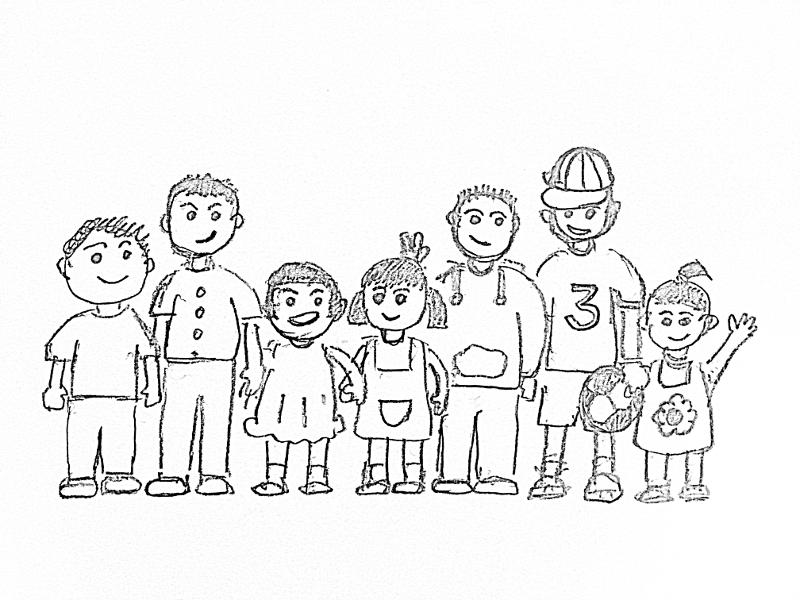
\includegraphics[scale=0.3]{img/kids.eps}
 \caption{安排小朋友们站成一队。}
 \label{fig:knuth-ssort}
\end{figure}

有很多方法可以做到,其中就包括快速排序的方法:

\begin{enumerate}
  \item 第一个小朋友举起手。所有比这个小朋友矮的都站到他的左侧去;所有比他高的站到他的右侧去;
  \item 所有站到左侧的小朋友重复这一步骤;所有站到右侧的小朋友也重复这一步骤。
\end{enumerate}

假设一组小朋友的身高为(单位是厘米):$\{102, 100, 98, 95, 96, 99, 101, 97\}$。下表描述了它们按照上述方法站队的过程。

\begin{tabular}{ | c c c c c c c c |}
\hline
\underline{102} & 100 & 98 & 95 & 96 & 99 & 101 & 97 \\
\underline{100} & 98 & 95 & 96 & 99 & 101 & 97 & `102' \\
\underline{98} & 95 & 96 & 99 & 97 & `100' & 101 & `102' \\
\underline{95} & 96 & 97 & `98' & 99 & `100' & `101' & `102' \\
`95' & \underline{96} & 97 & `98' & `99' & `100' & `101' & `102' \\
`95' & `96' & 97 & `98' & `99' & `100' & `101' & `102' \\
`95' & `96' & `97' & `98' & `99' & `100' & `101' & `102' \\
\hline
\end{tabular}

最开始的时候,身高为102厘米的第一个小朋友举手。我们称这个小朋友为pivot,并用下划线标记他。恰巧这个小朋友的身高是最高的。因此所有其他人都站到他的左侧,如表中第二行所示。此时,身高为102厘米的小朋友站到了最终应站的位置,所以我们用引号把他括起来。接下来身高为100里面的小朋友举手,因此,身高为98、95、96、和99厘米的小朋友站到了他的左侧,而只有一名身高为101厘米的小朋友身高比pivot高,所以他站到了右侧。表中的第三行给出了此时的状态。然后,身高为98厘米的小朋友成为了左侧的pivot;而身高为101厘米的小朋友成为了右侧的pivot。但是身高101厘米为pivot的那组小朋友只有他一个人,因此无需继续排序了。他站立的位置就是最终的位置。我们重复同样的方法,直到所有人都站到最终位置。

\subsection{基本形式}
\index{快速排序!基本形式}

归纳述步骤可以得到快速排序的递归描述。对序列$L$进行排序时:

\begin{itemize}
\item 若$L$为空,则排序结果明显为空。这是边界情况;
\item 否则,在$L$中任选一个元素作为pivot,然后递归地将$L$中不大于pivot的元素排序,将结果置于pivot的左侧,\underline{同时}递归地将所有大于pivot的元素排序,将结果置于pivot的右侧。
\end{itemize}

这里我们强调了“同时”,而不是“然后”。也就是说,左右两侧的递归排序是可以同时并行进行的。我们后面会再次讨论有关并行的内容。

快速排序由C. A. R. Hoare在1960年提出\cite{TAOCP}、\cite{wiki-qs}。这里给出的描述是最基本的一种。它并没有明确解释如何选择pivot。我们稍后会看到pivot的选取会直接影响到排序的性能。

最简单的方法是总选择第一个元素作为pivot。这样就可以将快速排序形式化为下面的公式:

\be
sort(L) = \left \{
  \begin{array}
  {r@{\quad:\quad}l}
  \phi & L = \phi \\
  sort(\{ x | x \in L', x \leq l_1 \}) \cup \{ l_1 \} \cup sort(\{ x | x \in L', l_1 < x \}) & otherwise \\
  \end{array}
\right.
\ee

其中$l_1$是非空序列$L$中的第一个元素,而$L'$包含除$l_1$外的剩余部分$\{l_2, l_3, ...\}$。这里我们使用了Zermelo Frankel表达式(简称为ZF表达式)\footnote{以纪念对现代集合论贡献巨大的两位数学家。中文译作:策梅罗、弗兰克尔。},也称为list comprehension。一个ZF表达式$\{ a | a \in S, p_1(a), p_2(a), ... \}$表示从集合$S$中选取使得断言$p_1, p_2, ...$都为真的元素。ZF表达式原本用于表示\underline{集合},我们将其扩展以简短地表示列表。因此允许存在重复的元素,并且不同的排列代表不同的列表。详细信息请参考本书的附录A。

在支持list comprehension的编程环境中,上述公式可以直接翻译为代码。如下面的Haskell例子程序:

\lstset{language=Haskell}
\begin{lstlisting}[style=Haskell]
sort [] = []
sort (x:xs) = sort [y | y<-xs, y <= x] ++ [x] ++ sort [y | y<-xs, x < y]
\end{lstlisting}

迄今为止,这可能是最短的快速排序程序。即使引入一些中间变量,程序也仍然简洁:

\lstset{language=Haskell}
\begin{lstlisting}[style=Haskell]
sort [] = []
sort (x:xs) = as ++ [x] ++ bs where
    as = sort [ a | a <- xs, a <= x]
    bs = sort [ b | b <- xs, x < b]
\end{lstlisting}

这一基本的快速排序程序还有一些变形,例如明确使用filter,而不是list comprehension。如下面的Python例子所示:

\lstset{language=Python}
\begin{lstlisting}
def sort(xs):
    if xs == []:
        return []
    pivot = xs[0]
    as = sort(filter(lambda x : x <= pivot, xs[1:]))
    bs = sort(filter(lambda x : pivot < x, xs[1:]))
    return as + [pivot] + bs
\end{lstlisting}

\subsection{严格弱序}
\index{快速排序!Strict weak ordering}

我们假设元素按照单调非递减的顺序排序。我们也可以改变算法,按照其他条件排序。这样就可以适用更多场景,在实际中,待排序的元素可能是数字、字符串、或者其他更复杂的内容(例如对一组列表排序)。

典型的方法,是把比较条件抽象成一个参数,如同此前在插入排序和选择排序的章节中所描述的。我们并不要求比较条件一定要遵从全序(total order),但是至少要满足\underline{严格弱序} (strict weak order)\cite{wiki-total-order}、\cite{wiki-sweak-order}。

简单起见,我们仅仅考虑使用小于等于(不大于)作为比较条件来进行排序。

\subsection{划分(Partition)}
\index{快速排序!partition}
观察前面的基本快速排序算法,会发现遍历了两次:第一次遍历获得了所有不大于pivot的元素,第二次遍历获得了所有大于pivot的元素。我们可以将他们合并成只遍历一次的划分过程。定义如下:

\be
partition(p, L) = \left \{
  \begin{array}
  {r@{\quad:\quad}l}
  (\phi, \phi) & L = \phi \\
  (\{ l_1 \} \cup A, B) & p(l_1), (A, B) = partition(p, L') \\
  (A, \{ l_1 \} \cup B) & \lnot p(l_1)
  \end{array}
\right.
\ee

这里的$\{x\} \cup L$仅仅是一个“cons”操作(将元素链接到表头),它只需要常数时间。使用partition,快速排序可以定义为:

\be
sort(L) = \left \{
  \begin{array}
  {r@{\quad:\quad}l}
  \phi & L = \phi \\
  sort(A) \cup \{l_1\} \cup sort(B) & L \neq \phi, (A, B) = partition(\lambda_x x \leq l_1, L')
  \end{array}
\right.
\ee

下面的Haskell例子程序实现了这一算法。

\lstset{language=Haskell}
\begin{lstlisting}[style=Haskell]
sort [] = []
sort (x:xs) = sort as ++ [x] ++ sort bs where
    (as, bs) = partition (<= x) xs

partition _ [] = ([], [])
partition p (x:xs) = let (as, bs) = partition p xs in
    if p x then (x:as, bs) else (as, x:bs)
\end{lstlisting}

划分(partition)的概念对于快速排序至关重要。划分在其很多其他排序排序算法中也很关键。本章的最后部分会解释它如何普遍地影响着排序的思想方法。在进一步改进快速排序的划分算法前,我们先来考虑如何用命令式的方法实现in-place的快速排序。

在诸多的划分方法中,Lomuto\cite{Bentley}、\cite{CLRS}给出的方法是最简单易懂的。我们稍后还会介绍其他划分方法,并展示不同的方法是如何影响性能的。

\begin{figure}[htbp]
   \centering
   \subfloat[划分的不变性质]{
      \begin{tikzpicture}[scale=0.8]
      \draw (0, 0) rectangle (1, 1) node (xl) [pos=.5] {x[l]}
            (1, 0) rectangle (5, 1) node (leq) [pos=.5] {...不大于pivot的...}
            (5, 0) rectangle (9, 1) node (ge) [pos=.5] {...大于pivot的...}
            (9, 0) rectangle (11, 1) node (rest) [pos=.5] {...?...}
            (11, 0) rectangle (12, 1) node (xu) [pos=.5] {x[u]};
      \fill [black] (5, 0) rectangle (5.1, 1) node (leftbar) [pos=.5] {}
                    (9, 0) rectangle (9.1, 1) node (rightbar) [pos=.5] {};
      \draw (0, 2) node (pivot) {pivot $p$}
            (5, 2) node (left) {左边界$L$}
            (9, 2) node (right) {右边界$R$};
      \draw[thick, ->] (pivot) edge (xl)
                       (left) edge [bend right] (leftbar)
                       (right) edge [bend right] (rightbar);
      \end{tikzpicture}} \\
   \subfloat[开始]{
      \begin{tikzpicture}[scale=0.8]
      \draw (-0.5, 0) rectangle (1, 1) node (xl) [pos=.5] {x[l]}
            (1, 0) rectangle (2.5, 1) node (xl1) [pos=.5] {x[l+1]}
            (2.5, 0) rectangle (4, 1) node (rest) [pos=.5] (ai) {...?...}
            (4, 0) rectangle (5, 1) node (xu) [pos=.5] {x[u]};
      \fill [black] (1, 0) rectangle (1.1, 1) node (leftbar) [pos=.5] {};
      \draw (-2, 2) node (pivot) {pivot $p$}
            (0, 2) node (left) {左边界$L$}
            (2, 2) node (right) {右边界$R$};
      \draw[thick, ->] (pivot) edge [bend right] (xl)
                       (left) edge [bend right] (leftbar)
                       (right) edge [bend left] (leftbar);
      \end{tikzpicture}} \\
   \subfloat[结束]{
      \begin{tikzpicture}[scale=0.8]
      \draw (0, 0) rectangle (1, 1) node (xl) [pos=.5] {x[l]}
            (1, 0) rectangle (5, 1) node (leq) [pos=.5] {...不大于pivot的...}
            (5, 0) rectangle (6, 1) node (xleft) [pos=.5] {x[$L$] }
            (6, 0) rectangle (10, 1) node (ge) [pos=.5] {...大于pivot的...}
            (10, 0) rectangle (11, 1) node (xu) [pos=.5] {x[u]};
      \fill [black] (6, 0) rectangle (6.1, 1) node (leftbar) [pos=.5] {}
                    (11, 0) rectangle (11.1, 1) node (rightbar) [pos=.5] {};
      \draw (0, 2) node (pivot) {pivot $p$}
            (6, 2) node (left) {左边界$L$}
            (12, 2) node (right) {右边界$R$};
      \draw[thick, ->] (pivot) edge (xl)
                       (left) edge [bend right] (leftbar)
                       (right) edge [bend left] (rightbar)
                       (xl) edge [bend right] node [below] {交换} (xleft);
      \end{tikzpicture}} \\
   \caption{使用最左边的元素作pivot划分一段数组。}
   \label{fig:partition-1-way}
\end{figure}

图\ref{fig:partition-1-way}描述了这种一次遍历进行划分的方法。我们从左向右逐一处理数组中的元素。任何时候,数组都由图\ref{fig:partition-1-way} (a)所示的几部分组成:

\begin{itemize}
\item 最左侧为pivot,当划分过程结束时,pivot会被移动到最终的位置;
\item 一段只包含不大于pivot的元素的部分。这一段的右侧边界被标记为$L$;
\item 一段只包含大于pivot的元素的部分。这一段的右侧边界被标记为$R$。也就是说,$L$标记和$R$标记之间的元素都大于pivot;
\item $R$标记后面的元素尚未被处理。这部分的元素可能大于,也可能不大于pivot。
\end{itemize}

在划分过程开始的时候,$L$标记指向pivot,$R$标记指向pivot后的下一个元素,如图\ref{fig:partition-1-way} (b)所示。然后算法不断地向右侧移动$R$标记进行处理直到$R$标记越过数组的右侧边界。

每次迭代,都比较$R$标记指向的元素和pivot的大小。若大于pivot,这一元素应该位于$L$和$R$标记之间,算法继续向前移动$R$标记以检查下一个元素;否则,说明$R$标记指向的元素小于或者等于pivot(不大于),它应该位于$L$标记的左侧。为此,我们将$L$标记向前移动一步,然后交换$L$和$R$标记指向的元素。

当$R$标记越过最后一个元素时,所有的元素都已处理完毕。大于pivot的元素都被移动到了$L$标记的右侧,而其他元素位于$L$标记的左侧。此时我们需要移动pivot元素,使得它位于这两段的中间。为此,我们可以交换pivot和$L$标记指向的元素。如图\ref{fig:partition-1-way} (c)中的双向箭头所示。

$L$标记最终指向pivot,它将整个的数组分成了两部分。我们将$L$标记作为划分过程的结果返回。实际中,为了方便后继处理,我们通常将$L$标记增加1,使得它指向第一个大于pivot的元素。整个划分过程中,我们in-place地修改了数组中的内容。

划分算法可以描述如下。它接受三个参数:一个数组$A$,待划分区间的上下界\footnote{这里描述的算法和\cite{CLRS}中的略有不同,后者用待划分区间的最后一个元素作为pivot。}

\begin{algorithmic}[1]
\Function{Partition}{A, l, u}
  \State $p \gets A[l]$  \Comment{$p$为pivot}
  \State $L \gets l$ \Comment{左侧标记}
  \For{$R \in [l+1, u]$} \Comment{对右侧标记进行迭代}
    \If{$\lnot (p < A[R])$} \Comment{对于严格弱序,定义$<$比较就足够了}
      \State $L \gets L + 1$
      \State \textproc{Exchange} $A[L] \leftrightarrow A[R]$
    \EndIf
  \EndFor
  \State \textproc{Exchange} $A[L] \leftrightarrow p$
  \State \Return $L + 1$ \Comment{返回划分的位置}
\EndFunction
\end{algorithmic}

下表给出了划分数组$\{ 3, 2, 5, 4, 0, 1, 6, 7\}$的步骤。

\begin{tabular}{|llllllll|l|}
\hline
\underline{3}(l)  & 2(r) & 5 & 4 & 0 & 1 & 6 & 7 & 开始,$pivot = 3$、$l = 1$、$r = 2$ \\
\underline{3} & 2(l)(r) & 5 & 4 & 0 & 1 & 6 & 7 & $2 < 3$,移动$l$($r=l$)\\
\underline{3} & 2(l) & 5(r) & 4 & 0 & 1 & 6 & 7 & $5 > 3$, 继续 \\
\underline{3} & 2(l) & 5 & 4(r) & 0 & 1 & 6 & 7 & $4 > 3$, 继续 \\
\underline{3} & 2(l) & 5 & 4 & 0(r) & 1 & 6 & 7 & $0 < 3$ \\
\underline{3} & 2 & 0(l) & 4 & 5(r) & 1 & 6 & 7 & 移动$l$,然后和$r$交换 \\
\underline{3} & 2 & 0(l) & 4 & 5 & 1(r) & 6 & 7 & $1 < 3$ \\
\underline{3} & 2 & 0 & 1(l) & 5 & 4(r) & 6 & 7 & 移动$l$,然后和$r$交换 \\
\underline{3} & 2 & 0 & 1(l) & 5 & 4 & 6(r) & 7 & $6 > 3$,继续 \\
\underline{3} & 2 & 0 & 1(l) & 5 & 4 & 6 & 7(r) & $7 > 3$,继续 \\
1 & 2 & 0 & 3 & 5(l+1) & 4 & 6 & 7 & $r$越过了边界,交换pivot和$l$ \\
\hline
\end{tabular}

下面的ANSI C例子程序实现了这一划分算法。

\lstset{language=C}
\begin{lstlisting}
int partition(Key* xs, int l, int u) {
    int pivot, r;
    for (pivot = l, r = l + 1; r < u; ++r)
        if (!(xs[pivot] < xs[r])) {
            ++l;
            swap(xs[l], xs[r]);
        }
    swap(xs[pivot], xs[l]);
    return l + 1;
}
\end{lstlisting}

其中\texttt{swap(a, b)}可以定义为函数或者宏。ISO C++中\texttt{swap(a, b)}在标准库中以函数模板的形式提供。被交换的元素类型通过模板进行推导。我们此后不再详细解释这些语言细节。

使用这一划分算法,命令式的in-place快速排序可以实现如下:

\begin{algorithmic}[1]
\Procedure{Quick-Sort}{$A, l, u$}
  \If{$l < u$}
    \State $m \gets$ \Call{Partition}{$A, l, u$}
    \State \Call{Quick-Sort}{$A, l, m - 1$}
    \State \Call{Quick-Sort}{$A, m, u$}
  \EndIf
\EndProcedure
\end{algorithmic}

对数组进行排序时,我们传入数组的上下界,如:\textproc{Quick-Sort}($A, 1, |A|$)。其中$l \geq u$用以判断数组片段为空或者只含有一个元素,这两种情况下我们都认为数组是已序的,算法直接返回而无需做任何处理。

下面的ANSI C例子程序给出了in-place快速排序的实现。

\lstset{language=C}
\begin{lstlisting}
void quicksort(Key* xs, int l, int u) {
    int m;
    if (l < u) {
        m = partition(xs, l, u);
        quicksort(xs, l, m - 1);
        quicksort(xs, m, u);
    }
}
\end{lstlisting}

\subsection{函数式划分算法的小改进}
\index{快速排序!One pass functional partition}

在深入分析快速排序的划分算法前,我们首先可以用fold来实现一个小改进:只需要遍历一遍就可以完成划分的算法。读者可以参考本书附录A来了解fold的详细内容。

\be
partition(p, L) = fold(f(p), (\phi, \phi), L)
\ee

其中函数$f$使用断言$p$来对元素和pivot进行比较。断言作为一个参数传入函数$f$,我们称之为$f$的“柯里化”形式(Currying form),参见附录A。另外,$f$可以是$partition$函数作用域内的一个词法闭包(lexical closure),它可以访问这一作用域内的断言。函数$f$不断更新划分结果内的一对列表。

\be
f(p, x, (A, B)) =  \left \{
  \begin{array}
  {r@{\quad:\quad}l}
  (\{ x \} \cup A, B) & p(x) \\
  (A, \{ x \} \cup B) & \lnot p(x)
  \end{array}
\right.
\ee

我们这里使用了模式匹配(pattern-matching)形式的定义。在不支持模式匹配的环境中,需要使用一个变量,如$P$来代表列表对$(A, B)$,并使用函数来获取$P$中的两个值。

下面的Haskell例子程序实现了这一改进的快速排序,每次划分只需要遍历一次。

\lstset{language=Haskell}
\begin{lstlisting}[style=Haskell]
sort [] = []
sort (x:xs) = sort small ++ [x] ++ sort big where
  (small, big) = foldr f ([], []) xs
  f a (as, bs) = if a <= x then (a:as, bs) else (as, a:bs)
\end{lstlisting}

\subsubsection{累积划分(Accumulated partition)}
\index{快速排序!Accmulated partition}

使用fold进行划分的过程,实际上是向结果列表对$(A, B)$累积的过程。若元素不大于pivot,则它被累积到$A$,否则累积到$B$。我们可以将这一累积过程明确定义出来,相对于最初的基本快速排序算法,这样既可以节省空间,又利于进行尾递归优化(参见附录A)。

\be
partition(p, L, A, B) = \left \{
  \begin{array}
  {r@{\quad:\quad}l}
  (A, B) & L = \phi \\
  partition(p, L', \{ l_1 \} \cup A, B) & p(l_1) \\
  partition(p, L', A, \{ l_1 \} \cup B) & otherwise
  \end{array}
\right.
\ee

其中,若列表$L$不空,则$l_1$代表其中的第一个元素,$L'$代表除第一元素外的剩余部分,形如:$L' = \{ l_2, l_3, ...\}$。通过向划分函数传入比较参数,如:$\lambda_x x \leq pivot$即可以实现升序的排序算法。

\be
sort(L) =  \left \{
  \begin{array}
  {r@{\quad:\quad}l}
  \phi & L = \phi \\
  sort(A) \cup \{ l_1 \} \cup sort(B) & otherwise
  \end{array}
\right.
\ee

其中$A$、$B$是通过上述划分函数计算出的结果。

\[
(A, B) = partition(\lambda_x x \leq l_1, L', \phi, \phi)
\]

\subsubsection{累积式快速排序}
\index{快速排序!Accumulated quick sort}

观察前面快速排序定义中的递归部分可以发现,列表的连接操作$sort(A) \cup \{l_1\} \cup sort(B)$需要的时间和列表的长度成比例。可以使用附录A中介绍的一些方法提高性能,另外,也可以将排序算法转换为累积形式。

\[
sort'(L, S) =  \left \{
  \begin{array}
  {r@{\quad:\quad}l}
  S & L = \phi \\
  ... & otherwise
  \end{array}
\right.
\]

其中$S$为累积结果。我们传入一个空的起始值来启动排序:$sort(L) = sort'(L, \phi)$。当划分完成时,需要递归地对两个子列表进行排序。我们可以先递归地将大于pivot的元素排序,然后将pivot链接到这一结果的前面。然后将链接结果作为新的“累积结果”传入后续的排序过程中。

根据这一思路,上述算法中的省略号部分可以实现如下:

\[
sort'(L, S) =  \left \{
  \begin{array}
  {r@{\quad:\quad}l}
  S & L = \phi \\
  sort(A, \{l_1\} \cup sort(B, ?)) & otherwise
  \end{array}
\right.
\]

当开始对$B$排序时,累积结果应该是什么呢?这里有一个很重要的不变性质:任何时候,累积结果$S$中总保存了迄今为止已经排序好的元素。因此,我们通过向$S$累积来对$B$排序。

\be
sort'(L, S) =  \left \{
  \begin{array}
  {r@{\quad:\quad}l}
  S & L = \phi \\
  sort(A, \{l_1\} \cup sort(B, S)) & otherwise
  \end{array}
\right.
\ee

下面的Haskell例子程序实现了累积式快速排序算法。

\lstset{language=Haskell}
\begin{lstlisting}[style=Haskell]
asort xs = asort' xs []

asort' [] acc = acc
asort' (x:xs) acc = asort' as (x:asort' bs acc) where
  (as, bs) = part xs [] []
  part [] as bs = (as, bs)
  part (y:ys) as bs | y <= x = part ys (y:as) bs
                    | otherwise = part ys as (y:bs)
\end{lstlisting}

\begin{Exercise}
\begin{itemize}
\item 选择一门命令式语言,实现递归的基本快速排序算法。
\item 和命令式快速排序算法类似,除了列表为空的情况外,如果列表只含有一个元素,也可以作为边界情况处理。修改函数式算法,处理这一边界情况。
\item 在累积式快速排序算法的实现中,使用了中间变量$A$、$B$。我们可以通过重新定义划分函数,通过递归调用sort函数来消除中间变量。选择一门函数式编程语言,实现这一改动。
\end{itemize}
\end{Exercise}

\section{快速排序的性能分析}
\index{快速排序!性能分析}

快速排序在实际应用中性能良好,但是给出严格的分析却并不容易。我们需要使用统计学工具来证明平均情况下的性能。

尽管如此,我们可以很直观地计算出最好情况和最坏情况下的性能。显然,最好情况发生在每次划分都能将序列均分成两段长度相同子序列时。如图\ref{fig:qsort-best}所示,共需要$O(\lg n)$次递归调用。

\begin{figure}[htbp]
 \centering
 \includegraphics[scale=0.6]{img/qsort-best.ps}
 \caption{最好情况下,快速排序每次将序列划分成长度相等的两部分。}
 \label{fig:qsort-best}
\end{figure}

总共有$O(\lg n)$层递归。在第一层,进行一次划分,处理$n$个元素;在第二层,进行两次划分,每次划分处理$n/2$个元素,第二层的总体执行时间为$2 O(n/2) = O(n)$。在第三层,执行划分四次,每次处理$n/4$个元素,第三层的总体执行时间也是$O(n)$……在最后一层,总共有$n$个片段,每个片段只含有一个元素,总处理时间也是$O(n)$。将上述所有层的执行时间相加,得到快速排序在最好情况下的性能为$O(n \lg n)$。

但是在最坏情况下,划分过程大部分时间都把序列分成两个很不平衡的部分。其中一部分的长度为$O(1)$,另一部分的长度为$O(n)$。因此递归的深度退化为$O(n)$。如果我们用同样的图来描述,最好情况下,快速排序过程形成一棵平衡二叉树;而最坏情况下,会形成一棵很不平衡的树,每个节点都只有一棵子树,而另外一棵子树为空。二叉树退化成了一个长度为$O(n)$的链表。而在每一层中,所有的元素都被处理,因此最坏情况下的性能为$O(n^2)$,这和插入排序、选择排序的性能相当。

最坏情况在何时发生的?其中一个特殊情况是所有的元素(或大部分元素)都相同。Lomuto的划分方法此时的表现很差。我们在下一节会介绍另外一种划分方法,可以有效解决这一问题。

另外有两种明显的序列类型可以导致最坏情况:即序列已序(升序或降序)。划分升序序列时pivot前的部分总是空的,而pivot后的部分包含所有剩余元素。划分降序序列的结果与此相反。

还有其他一些情况可以导致快速排序的性能很差。不存在一种方法可以完全避免最坏情况。我们下一节会给出一些工程方法可以把最坏情况发生的可能性降低。

\subsection{平均情况的分析 $\star$}
\index{快速排序!平均情况分析}

快速排序在平均情况下性能良好。甚至在每次划分时,总得到长度比为1:9的两部分,总体性能仍然为$O(n \lg n)$\cite{CLRS}。

本节需要一些额外的数学知识,读者可以选择跳过。

有两种方法可以证明快速排序在平均情况下的性能。其中一种方法利用了快速排序中的比较操作的次数来考量性能\cite{CLRS}。例如,在选择排序中,任何两个元素都进行了比较。而快速排序却避免了很多不必要的比较。考虑划分列表$\{ a_1, a_2, a_3, ..., a_n\}$,选择$a_1$作为pivot,划分结果产生两个子列表$A = \{x_1, x_2, ..., x_k\}$和$B = \{ y_1, y_2, ..., y_{n-k-1} \}$。在接下来的快速排序过程中,$A$中的任何元素,都不再和$B$中的任何元素进行比较。

记最终排序的结果为$\{ a_1, a_2, ..., a_n \}$,我们有这样的结果:若$a_i < a_j$,当且仅当存在某一元素$a_k$满足$a_i < a_k < a_j$,并且$a_k$在$a_i$或$a_j$之前被选为pivot时,我们将不再对$a_i$和$a_j$进行比较。

也就是说,$a_i$与$a_j$进行比较的唯一可能是要么$a_i$,要么$a_j$在所有$a_{i+1} < a_{i+2} < ... < a_{j-1}$之前被选为pivot。

令$P(i, j)$代表$a_i$和$a_j$进行比较的概率,我们有:

\be
P(i, j) = \frac{2}{j - i + 1}
\ee

全部比较操作的总数可以这样得到:

\be
C(n) = \sum_{i=1}^{n-1}\sum_{j=i+1}^{n} P(i, j)
\ee

如果我们比较了$a_i$和$a_j$,在接下来的快速排序中,就不再比较$a_j$和$a_i$,并且元素$a_i$永远不会和自己进行比较。因此在上式中,$i$的上限为$n-1$,$j$的下限为$i+1$。

将概率代入,得:

\be
\begin{array}{rl}
C(n) & = \displaystyle \sum_{i=1}^{n-1}\sum_{j = i+1}^{n} \frac{2}{j - i + 1} \\
     & = \displaystyle \sum_{i=1}^{n-1}\sum_{k=1}^{n-i} \frac{2}{k+1} \\
\end{array}
\ee

使用调和级数\cite{wiki-harmonic}。

\[
H_n = 1 + \frac{1}{2} + \frac{1}{3} + .... = \ln n + \gamma + \epsilon_n
\]

因此:

\be
C(n) = \sum_{i=1}^{n-1} O(\lg n) = O(n \lg n)
\ee

我们还可以用另外一种方法证明快速排序在平均情况下的性能。考虑递归,当待排序的列表长度为$n$时,划分过程将列表分成两个部分,一部分长度为$i$,另一部分长度为$n-i-1$。划分过程需要比较pivot和每个元素,它自身用时$cn$。因此我们有如下递归关系:

\be
T(n) = T(i) + T(n-i-1) + c n
\ee

其中$T(n)$是对长度为$n$的列表进行快速排序所用的时间。由于$i$以相同的概率在$0, 1, ..., n-1$中取值,通过使用数学期望,可以得到如下结果:

\be
\renewcommand*{\arraystretch}{1.5}
\begin{array}{rl}
T(n) & = E(T(i)) + E(T(n-i-1)) + c n \\
     & = \displaystyle \frac{1}{n} \sum_{i=0}^{n-1}T(i) + \frac{1}{n} \sum_{i=0}^{n-1}T(n-i-1) + cn \\
     & = \displaystyle \frac{1}{n} \sum_{i=0}^{n-1}T(i) + \frac{1}{n} \sum_{j=0}^{n-1}T(j) + cn \\
     & = \displaystyle \frac{2}{n} \sum_{i=0}^{b-1}T(i) + cn
\end{array}
\ee

两边同时乘以$n$:

\be
n T(n) = 2 \sum_{i=0}^{n-1} T(i) + c n^2
\label{eq:ntn}
\ee

将$n$用$n-1$替换,可以得到另外一个等式:

\be
(n-1) T(n-1) = 2 \sum_{i=0}^{n-2} T(i) + c (n-1)^2
\label{eq:n1tn1}
\ee

用式(\ref{eq:ntn})减去式(\ref{eq:n1tn1})可以消去所有的$T(i)$,其中$0 \leq i < n-1$。

\be
n T(n) = (n + 1) T(n-1) + 2cn - c
\ee

在计算性能时,我们可以忽略掉常数时间$c$。因此上式进一步变化为:

\be
\frac{T(n)}{n+1} = \frac{T(n-1)}{n} + \frac{2c}{n+1}
\ee

我们依次用$n-1$、$n-2$……代入$n$,可以得到$n-1$个等式。

\[
\frac{T(n-1)}{n} = \frac{T(n-2)}{n-1} + \frac{2c}{n}
\]

\[
\frac{T(n-2)}{n-1} = \frac{T(n-3)}{n-2} + \frac{2c}{n-1}
\]

\[
...
\]

\[
\frac{T(2)}{3} = \frac{T(1)}{2} + \frac{2c}{3}
\]

将所有等式相加,消去左右两侧相同的变量,可以化简得到一个关于$n$的函数。

\be
\frac{T(n)}{n+1} = \frac{T(1)}{2} + 2c \sum_{k=3}^{n+1} \frac{1}{k}
\ee

使用上面提到的调和级数,最终的结果为:

\be
O(\frac{T(n)}{n+1}) = O(\frac{T(1)}{2} + 2c \ln n + \gamma + \epsilon_n) = O(\lg n)
\ee

因此

\be
O(T(n)) = O(n \lg n)
\ee

\begin{Exercise}
\begin{itemize}
\item 当有很多重复元素时,为什么Lomuto的方法性能会变差?
\end{itemize}
\end{Exercise}

% ================================================================
% Minor Improvement for quick sort
% ================================================================

\section{工程实践中的改进}
\index{快速排序!Engineering improvement}

大多数情况下快速排序性能优异。但是在最差的情况下,性能会下降到平方级别。如果待排序的数据是完全随机分布的,出现最差情况的概率会很低。尽管如此,某些常见的特殊序列却仍会引发最差情况。

本节我们介绍一些工程上常用的方法,它们或者针对某些特殊的输入数据改进划分算法来避免性能下降,或者通过改变概率分布来减小出现最差情况的可能。

\subsection{处理重复元素的工程方法}
\index{快速排序!处理重复元素}

如上一节的练习中所示,Lomuto的划分算法不擅长处理含有很多重复元素的序列。考虑含有$n$个相等元素的特殊序列$\{x, x, ..., x\}$,我们有两种方案来进行排序。

\begin{enumerate}
\item 普通的基本快速排序法:我们任意选择一个元素作为pivot,其值为$x$,这样分割后得到两个子序列,一个是$\{x, x, ..., x \}$,包含$n-1$个元素,另外一个子序列为空。接下来递归地对第一个子序列排序;这明显是一个$O(n^2)$的解决方法。
\item 另外一个方法是只挑选严格小于$x$的元素,和严格大于$x$的元素进行划分。这样得到的结果是两个空序列,和$n$个等于pivot的元素。接下来我们递归地对只含有小于pivot的元素子序列和只含有大于pivot的元素的子序列进行排序,由于它们都为空,因此递归调用立即结束。剩下要做的就是将比pivot小的元素的排序结果,全部等于pivot的元素,和比pivot大的元素的排序结果连接起来。
\end{enumerate}

如果所有元素都相等,第二种方法只需要$O(n)$时间。这给出了划分算法的一个重要改进:相对于二分划分(binary partition,划分成两个子序列和一个pivot),三分划分(ternary partition,划分成三个子序列)能更好地处理重复元素。

我们可以这样来定义三分划分快速排序(ternary quick sort):

\be
sort(L) = \left \{
  \begin{array}
  {r@{\quad:\quad}l}
  \phi & L = \phi \\
  sort(S) \cup sort(E) \cup sort(G) & otherwise
  \end{array}
\right.
\ee

其中$S, E, G$分别是所有小于、等于、和大于pivot的元素组成的列表。

\[
\begin{array}{l}
S = \{ x | x \in L, x < l_1 \} \\
E = \{ x | x \in L, x = l_1 \} \\
G = \{ x | x \in L, l_1 < x \}
\end{array}
\]

下面的Haskell例子程序实现了基本的三分快速排序算法。

\lstset{language=Haskell}
\begin{lstlisting}[style=Haskell]
sort [] = []
sort (x:xs) = sort [a | a<-xs, a<x] ++
              x:[b | b<-xs, b==x] ++ sort [c | c<-xs, c>x]
\end{lstlisting}

注意,元素间的比较必须支持“小于”和“等于”操作,而普通快速排序仅仅要求“小于”比较。在性能上,基本的三分快速排序需要线性时间$O(n)$将三个子列表连接起来。可以使用一个累积变量(accumulator)来改善这一性能。

令函数$sort'(L, A)$表示带有累积变量的三分快速排序定义,其中$L$为待排序序列,累积变量$A$包含已排好序的部分。它最开始时为空:$sort(L) = sort'(L, \phi)$。我们可以先定义好边界条件:

\[
sort'(L, A) = \left \{
  \begin{array}
  {r@{\quad:\quad}l}
  A & L = \phi \\
  ... & otherwise
  \end{array}
\right.
\]

对于递归情况,三分划分将序列分为三个子序列$S, E, G$,其中只有$S$和$G$需要递归排序,而$E$包含全部等于pivot的元素,无需进一步排序了。我们可以先使用累积变量$A$对$G$进行排序,然后将排序结果连接到$E$的后面,作为新的累积变量对$S$进行排序。

\be
sort'(L, A) = \left \{
  \begin{array}
  {r@{\quad:\quad}l}
  A & L = \phi \\
  sort(S, E \cup sort(G, A)) & otherwise
  \end{array}
\right.
\ee

划分算法也可以使用累积变量来实现。这和基本的快速排序类似。注意这里我们不能只传入一个和pivot进行比较的断言,而需要传入两个:一个用于“小于”比较,另外一个用于“等于”判断。简单起见,这里我们传入pivot元素。

\be
partition(p, L, S, E, G) = \left \{
  \begin{array}
  {r@{\quad:\quad}l}
  (S, E, G) & L = \phi \\
  partition(p, L', \{l_1\} \cup S, E, G) & l_1 < p \\
  partition(p, L', S, \{l_1\} \cup E, G) & l_1 = p \\
  partition(p, L', S, E, \{ l_1 \} \cup G) & p < l_1
  \end{array}
\right.
\ee

其中,若$L$不为空,$l_1$为$L$中的第一个元素,$L'$包含除$l_1$外的剩余部分。下面的Haskell例子程序实现了这一算法。它在划分算法的边界情况中启动递归排序。

\lstset{language=Haskell}
\begin{lstlisting}[style=Haskell]
sort xs = sort' xs []

sort' []     r = r
sort' (x:xs) r = part xs [] [x] [] r where
    part [] as bs cs r = sort' as (bs ++ sort' cs r)
    part (x':xs') as bs cs r | x' <  x = part xs' (x':as) bs cs r
                             | x' == x = part xs' as (x':bs) cs r
                             | x' >  x = part xs' as bs (x':cs) r
\end{lstlisting}

Richard Bird给出了另外一个改进\cite{fp-pearls},它不对递归排序的结果立即执行连接操作,而是把排好的子列表放入一个列表中保存。最终再将这些子列表连接在一起。

\lstset{language=Haskell}
\begin{lstlisting}[style=Haskell]
sort xs = concat $ pass xs []

pass [] xss = xss
pass (x:xs) xss = step xs [] [x] [] xss where
    step [] as bs cs xss = pass as (bs:pass cs xss)
    step (x':xs') as bs cs xss | x' <  x = step xs' (x':as) bs cs xss
                               | x' == x = step xs' as (x':bs) cs xss
                               | x' >  x = step xs' as bs (x':cs) xss
\end{lstlisting} %$

\subsubsection{双向划分(2-way partition)}
\index{快速排序!双向划分}

也可以用命令式的方法解决大量重复元素的问题。Robert Sedgewick给出了一个划分方法\cite{qsort-impl}、\cite{Bentley},使用两个指针,一个从左向右移动,另一个从右向左移动。开始的时候两个指针指向数组的左右边界。

划分开始时,选择最左侧的元素作为pivot。然后左侧指针$i$不断向右前进直到遇到一个不小于pivot的元素;另外\footnote{注意,我们没有使用“然后”一词,因为这两轮扫描可以同时并发进行。},右侧指针$j$不断向左扫描直到遇到一个不大于pivot的元素。

此时,所有在左侧指针$i$之前的元素都严格小于pivot,而所有在右侧指针$j$之后的元素都严格大于pivot。$i$指向一个大于或等于pivot的元素;而$j$指向一个小于或等于pivot的元素。图\ref{fig:partition-2-way} (a)描述了此时的情形。

为了将全部小于或等于pivot的元素划分到左侧,而其余元素划分到右侧,我们可以交换$i$和$j$指向的两个元素。然后我们恢复扫描,重复上面的步骤直到$i$和$j$相遇或者交错。

在划分的任何时刻,总保持着不变条件(invariant),即所有$i$之前的元素(包括$i$指向的元素)都不大于pivot;而所有$j$之后的元素(包括$j$指向的元素)都不小于pivot。$i$和$j$之间的元素尚未处理。图\ref{fig:partition-2-way} (b)描述了这一不变条件。

\begin{figure}[htbp]
   \centering
   \subfloat[指针$i$和$j$停止前进时]{
      \begin{tikzpicture}[scale=0.8]
      \draw (0, 0) rectangle (1, 1) node (xl) [pos=.5] {x[l]}
            (1, 0) rectangle (5, 1) node (leq) [pos=.5] {...小于pivot的...}
            (5, 0) rectangle (6, 1) node (xi) [pos=.5] {x[i]}
            (6, 0) rectangle (8, 1) node (rest) [pos=.5] {...?...}
            (8, 0) rectangle (9, 1) node (xj) [pos=.5] {x[j]}
            (9, 0) rectangle (13, 1) node (ge) [pos=.5] {...大于pivot的...};
      \draw (0, 2) node (pivot) {pivot $p$}
            (5, 2) node (left) {$\geq$ pivot}
            (8, 2) node (right) {$\leq$ pivot};
      \draw[thick, ->] (pivot) edge (xl)
                       (left) edge [bend right] (xi)
                       (right) edge [bend right] (xj);
      \end{tikzpicture}} \\
   \subfloat[划分不变条件]{
      \begin{tikzpicture}[scale=0.8]
      \draw (0, 0) rectangle (1, 1) node (xl) [pos=.5] {x[l]}
            (1, 0) rectangle (5, 1) node (leq) [pos=.5] {...不大于于pivot的...}
            (5, 0) rectangle (7, 1) node (rest) [pos=.5] {...?...}
            (7, 0) rectangle (11, 1) node (ge) [pos=.5] {...不小于pivot的...};
      \fill [black] (5, 0) rectangle (5.1, 1) node (ibar) [pos=.5] {}
                    (7, 0) rectangle (7.1, 1) node (jbar) [pos=.5] {};
      \draw (0, 2) node (pivot) {pivot $p$}
            (5, 2) node (i) {$i$}
            (7, 2) node (j) {$j$};
      \draw[thick, ->] (pivot) edge (xl)
                       (i) edge [bend right] (ibar)
                       (j) edge [bend right] (jbar);
      \end{tikzpicture}} \\
   \caption{选择最左侧的元素作为pivot进行划分。}
   \label{fig:partition-2-way}
\end{figure}

当左侧指针$i$和右侧指针$j$相遇或交错时,我们需要进行一次额外的交换操作,将最左侧的pivot元素交换到$j$指向的位置上。然后,我们对划分区间下界和$j$之间的数组片段,以及$i$和划分区间上界之间的片段进行递归排序。

这一算法可以描述如下。

\begin{algorithmic}[1]
\Procedure{Sort}{$A, l, u$} \Comment{sort range $[l, u)$}
  \If{$u - l > 1$} \Comment{非平凡情况下包含1个以上的元素}
    \State $i \gets l$, $j \gets u$
    \State $pivot \gets A[l]$
    \Loop
      \Repeat
        \State $i \gets i + 1$
      \Until{$A[i] \geq pivot$} \Comment{忽略$i \geq u$的错误处理}
      \Repeat
        \State $j \gets j - 1$
      \Until{$A[j] \leq pivot$} \Comment{忽略$j < l$的错误处理}
      \If{$j < i$}
        \State break
      \EndIf
      \State \textproc{Exchange} $A[i] \leftrightarrow A[j]$
    \EndLoop
    \State \textproc{Exchange} $A[l] \leftrightarrow A[j]$ \Comment{移动pivot}
    \State \Call{Sort}{$A, l, j$}
    \State \Call{Sort}{$A, i, u$}
  \EndIf
\EndProcedure
\end{algorithmic}

考虑所有元素都相等的极端情况,这一in-place的快速排序将数组划分为两段长度相等的子数组,这里发生了$\frac{n}{2}$次不必要的交换操作。由于划分是平衡的,所以总体性能仍然为$O(n \lg n)$,而没有下降到平方级别。下面的C语言例子程序实现了这一算法。

\lstset{language=C}
\begin{lstlisting}
void qsort(Key* xs, int l, int u) {
    int i, j, pivot;
    if (l < u - 1) {
        pivot = i = l; j = u;
        while (1) {
            while (i < u && xs[++i] < xs[pivot]);
            while (j >=l && xs[pivot] < xs[--j]);
            if (j < i) break;
            swap(xs[i], xs[j]);
        }
        swap(xs[pivot], xs[j]);
        qsort(xs, l, j);
        qsort(xs, i, u);
    }
}
\end{lstlisting}

和此前介绍的Lomuto的划分算法相比,可以发现这一算法的元素交换操作次数更少。这是因为它跳过了那些最终位置在pivot正确一侧的元素不进行交换。

\subsubsection{三路划分}
\index{快速排序!三路划分}

显然,我们应该避免对重复元素进行不必要的交换操作。进一步,可以利用“三分排序”(ternary sort,也称作三路划分)的思路来改进算法,所有严格小于pivot的元素被放入左侧的子序列片段,严格大于pivot的元素被放入右侧,而中间部分包含所有等于pivot的元素。使用三路划分,我们只需要对不等于pivot的元素进行递归排序。在上述的特殊情况中,由于所有的元素都相等,我们无需进行进一步的递归排序。因此整体的性能为线性时间$O(n)$。

我们接下来需要考虑如何实现三路划分。Jon Bentley和Douglas McIlroy给出了一个方法:如图\ref{fig:partition-3-way} (a)所示,所有和pivot相等的元素最初保存在最左侧和最右侧\cite{3-way-part}、\cite{opt-qs}。

\begin{figure}[htbp]
   \centering
   \subfloat[三路划分的不变条件。]{
      \begin{tikzpicture}[scale=0.8]
      \draw (0, 0) rectangle (1, 1) node (xl) [pos=.5] {x[l]}
            (1, 0) rectangle (3, 1) node [pos=.5] {...等于...}
            (3, 0) rectangle (5, 1) node [pos=.5] {...小于...}
            (5, 0) rectangle (7, 1) node [pos=.5] {...?...}
            (7, 0) rectangle (9, 1) node [pos=.5] {...大于...}
            (9, 0) rectangle (11, 1) node [pos=.5] {...等于...};
      \fill [black] (3, 0) rectangle (3.1, 1) node (pbar) [pos=.5] {}
                    (5, 0) rectangle (5.1, 1) node (ibar) [pos=.5] {}
                    (7, 0) rectangle (7.1, 1) node (jbar) [pos=.5] {}
                    (9, 0) rectangle (9.1, 1) node (qbar) [pos=.5] {};
      \draw (0, 2) node (pivot) {pivot}
            (3, 2) node (p) {$p$}
            (5, 2) node (i) {$i$}
            (7, 2) node (j) {$j$}
            (9, 2) node (q) {$q$};
      \draw[thick, ->] (pivot) edge (xl)
                       (p) edge [bend right] (pbar)
                       (i) edge [bend right] (ibar)
                       (j) edge [bend left] (jbar)
                       (q) edge [bend left] (qbar);
      \end{tikzpicture}} \\
   \subfloat[将和pivot相等的元素交换到中间部分。]{\hspace{0.1\textwidth}
      \begin{tikzpicture}[scale=0.8]
      \draw (0, 0) rectangle (2, 1) node [pos=.5] {...小于...}
            (2, 0) rectangle (4, 1) node [pos=.5] {...等于...}
            (4, 0) rectangle (6, 1) node [pos=.5] {...大于...};
      \fill [black] (2, 0) rectangle (2.1, 1) node (ibar) [pos=.5] {}
                    (4, 0) rectangle (4.1, 1) node (jbar) [pos=.5] {};
      \draw (2, 2) node (i) {$i$}
            (4, 2) node (j) {$j$};
      \draw[thick, ->] (i) edge [bend right] (ibar)
                       (j) edge [bend left] (jbar);
      \end{tikzpicture}
      \hspace{0.1\textwidth}}
   \caption{三路划分}
   \label{fig:partition-3-way}
\end{figure}

扫描过程大部分和Robert Sedgewick给出的相似,两个指针$i$和$j$相向前进直到$i$遇到任何大于等于pivot的元素,并且$j$遇到任何小于等于pivot的元素。此时,如果$i$和$j$没有相遇或者交错,我们不仅交换它们指向的元素,同时检查被指向的元素是否和pivot相等,如果相等,就交换$i$和$p$指向的元素,以及$j$和$q$指向的元素。

在划分过程结束前,需要把所有等于pivot的元素从左右两侧交换到中间。交换的次数取决于重复元素的个数。如果所有的元素都不等,则交换次数为零,不产生任何额外的性能消耗。划分的最终结果如图\ref{fig:partition-3-way} (b)所示。此后,我们只需要对“严格小于”和“严格大于”部分的子片段进行递归排序。

可以通过修改两路划分的算法进行实现。

\begin{algorithmic}[1]
\Procedure{Sort}{$A, l, u$}
  \If{$u - l > 1$}
    \State $i \gets l$, $j \gets u$
    \State $p \gets l$, $q \gets u$ \Comment{指向相等元素的边界}
    \State $pivot \gets A[l]$
    \Loop
      \Repeat
        \State $i \gets i + 1$
      \Until{$A[i] \geq pivot$} \Comment{忽略$i \geq u$的错误处理}
      \Repeat
        \State $j \gets j - 1$
      \Until{$A[j] \leq pivot$} \Comment{忽略$j < l$的错误处理}
      \If{$j \leq i$}
        \State break \Comment{注意和此前算法的不同}
      \EndIf
      \State \textproc{Exchange} $A[i] \leftrightarrow A[j]$
      \If{$A[i] = pivot$} \Comment{处理相等的元素}
        \State $p \gets p + 1$
        \State \textproc{Exchange} $A[p] \leftrightarrow A[i]$
      \EndIf
      \If{$A[j] = pivot$}
        \State $q \gets q - 1$
        \State \textproc{Exchange} $A[q] \leftrightarrow A[j]$
      \EndIf
    \EndLoop
    \If{$i = j \land A[i] = pivot$} \Comment{特殊情况}
      \State $j \gets j - 1$, $i \gets i + 1$
    \EndIf
    \For{$k$ from $l$ to $p$} \Comment{将相等的元素交换到中间}
      \State \textproc{Exchange} $A[k] \leftrightarrow A[j]$
      \State $j \gets j - 1$
    \EndFor
    \For{$k$ from $u-1$ down-to $q$}
      \State \textproc{Exchange} $A[k] \leftrightarrow A[i]$
      \State $i \gets i + 1$
    \EndFor
    \State \Call{Sort}{$A, l, j + 1$}
    \State \Call{Sort}{$A, i, u$}
  \EndIf
\EndProcedure
\end{algorithmic}

下面的C语言例子程序实现了三路划分快速排序算法。

\lstset{language=C}
\begin{lstlisting}
void qsort2(Key* xs, int l, int u) {
    int i, j, k, p, q, pivot;
    if (l < u - 1) {
        i = p = l; j = q = u; pivot = xs[l];
        while (1) {
            while (i < u && xs[++i] < pivot);
            while (j >= l && pivot < xs[--j]);
            if (j <= i) break;
            swap(xs[i], xs[j]);
            if (xs[i] == pivot) { ++p; swap(xs[p], xs[i]); }
            if (xs[j] == pivot) { --q; swap(xs[q], xs[j]); }
        }
        if (i == j && xs[i] == pivot) { --j, ++i; }
        for (k = l; k <= p; ++k, --j) swap(xs[k], xs[j]);
        for (k = u-1; k >= q; --k, ++i) swap(xs[k], xs[i]);
        qsort2(xs, l, j + 1);
        qsort2(xs, i, u);
    }
}
\end{lstlisting}

引入三路划分后,算法逐渐变得复杂了。各种边界条件都需要进行仔细的处理。回顾此前的Lomuto的划分方法,它的优势就是简单直观,我们可以考虑对它加以改进,得到一个简单的三路划分实现。

我们需要调整一下不变条件(invariant)。我们仍然选择第一个元素作为pivot,如图\ref{fig:partition-3-way-lomuto}所示,任何时刻,左侧的片段包含严格小于pivot的元素;接下来的片段包含等于pivot的元素;最右侧的片段包含严格大于pivot的元素。这三个片段的边界分别为$i$、$k$和$j$。剩余在$k$和$j$之间的部分是尚未扫描的元素。

我们从左向右逐一扫描元素,一开始时,严格小于pivot的部分为空;等于pivot的部分只包含一个元素,就是pivot本身。$i$此时指向数组的下界,$k$指向$i$的下一个元素。严格大于pivot的部分也为空,$j$指向数组的上界。

\begin{figure}[htbp]
   \centering
      \begin{tikzpicture}[scale=0.8]
      \draw (0, 0) rectangle (2, 1) node [pos=.5] {...小于...}
            (2, 0) rectangle (4, 1) node [pos=.5] {...等于...}
            (4, 0) rectangle (6, 1) node [pos=.5] {...?...}
            (6, 0) rectangle (8, 1) node [pos=.5] {...大于...};
      \fill [black] (2, 0) rectangle (2.1, 1) node (ibar) [pos=.5] {}
                    (4, 0) rectangle (4.1, 1) node (kbar) [pos=.5] {}
                    (6, 0) rectangle (6.1, 1) node (jbar) [pos=.5] {};
      \draw (2, 2) node (i) {$i$}
            (4, 2) node (k) {$k$}
            (6, 2) node (j) {$j$};
      \draw[thick, ->] (i) edge [bend right] (ibar)
                       (k) edge [bend right] (kbar)
                       (j) edge [bend left] (jbar);
      \end{tikzpicture}
   \caption{基于Lomuto方法的三路划分。}
   \label{fig:partition-3-way-lomuto}
\end{figure}

划分过程开始后,我们逐一检查$k$指向的元素。如果它等于pivot,$k$就移动指向下一个元素;如果它大于pivot,我们将它和未处理区间的最后一个元素交换,这样严格大于的区间长度就增加一。它的边界$j$向左移动一步。由于我们不确定移动到$k$的元素是否仍然大于pivot,我们需要再次进行比较,重复上述过程。否则,如果元素小于pivot,我们将它和等于pivot区间的第一个元素交换。当$k$和$j$相遇时,划分过程结束。

\begin{algorithmic}[1]
\Procedure{Sort}{$A, l, u$}
  \If{$u - l > 1$}
    \State $i \gets l$, $j \gets u$, $k \gets l + 1$
    \State $pivot \gets A[i]$
    \While{$k < j$}
      \While{$pivot < A[k]$}
        \State $j \gets j - 1$
        \State \textproc{Exchange} $A[k] \leftrightarrow A[j]$
      \EndWhile
      \If{$A[k] < pivot$}
        \State \textproc{Exchange} $A[k] \leftrightarrow A[i]$
        \State $i \gets i + 1$
      \EndIf
      \State $k \gets k + 1$
    \EndWhile
    \State \Call{Sort}{$A, l, i$}
    \State \Call{Sort}{$A, j, u$}
  \EndIf
\EndProcedure
\end{algorithmic}

和前面的三路划分快速排序算法相比,这一算法要相对简单,但是需要更多的交换次数。下面的C语言例子程序实现了这一算法。

\lstset{language=C}
\begin{lstlisting}
void qsort(Key* xs, int l, int u) {
    int i, j, k; Key pivot;
    if (l < u - 1) {
        i = l; j = u; pivot = xs[l];
        for (k = l + 1; k < j; ++k) {
            while (pivot < xs[k]) { --j; swap(xs[j], xs[k]); }
            if (xs[k] < pivot) { swap(xs[i], xs[k]); ++i; }
        }
        qsort(xs, l, i);
        qsort(xs, j, u);
    }
}
\end{lstlisting}

\begin{Exercise}
\begin{itemize}
\item 我们给出的命令式快速排序算法都使用第一个元素作为pivot,也可以使用最后一个元素作为pivot。请修改快速的排序的基本算法,Sedgewick的改进算法,和三路快速排序算法,使用最后一个元素作为pivot。
\end{itemize}
\end{Exercise}

\section{针对最差情况的工程实践}

虽然三分快速排序(使用三路划分)能处理含有很多重复元素的序列,但是仍然无法有效解决典型的最差情况。例如,如果序列中的大部分元素已序时,无论是升序还是降序,划分的结果将会是两个长度不平衡的子序列,一个包含少量的元素,另一个包含剩余的部分。

考虑两种极端情况:$\{ x_1 < x_2 < ... < x_n\}$和$\{ y_1 > y_2 > ... > y_n\}$。图\ref{fig:worst-cases-1}给出了划分结果。

\begin{figure}[htbp]
   \centering
   \subfloat[序列$\{x_1 < x_2 < ... < x_n\}$的划分树,每次划分时,选择第一个元素为pivot,小于等于pivot的部分总为空。]{\hspace{.3\textwidth} \includegraphics[scale=0.5]{img/unbalanced.ps} \hspace{.3\textwidth}} \\
   \subfloat[序列$\{y_1 > y_2 > ... > y_n\}$的划分树,每次划分时,选择第一个元素为pivot,大于等于pivot的部分总为空。]{\includegraphics[scale=0.5]{img/unbalanced-2.ps}} \\
   \caption{两种最差情况。}
   \label{fig:worst-cases-1}
\end{figure}

很容易给出更多的最差情况,例如$\{ x_m, x_{m-1}, ..., x_2, x_1, x_{m+1}, x_{m+2}, ... x_n\}$,其中$\{ x_1 < x_2 < ... < x_n \}$;另一个例子是$\{x_n, x_1, x_{n-1}, x_2, ... \}$。图\ref{fig:worst-cases-2}给出了它们的划分结果。

\begin{figure}[htbp]
   \centering
   \subfloat[除了第一次划分结果,其他都不平衡。]{\includegraphics[scale=0.4]{img/unbalanced-3.ps}} \\
   \subfloat[一个zig-zag形状的划分树。]{\includegraphics[scale=0.5]{img/unbalanced-zigzag.ps}} \\
   \caption{另两种最差情况。}
   \label{fig:worst-cases-2}
\end{figure}

观察可以发现,仅仅简单地选择第一个元素作为pivot,很容易使得划分的结果不平衡,Robert Sedgwick在\cite{qsort-impl}中给出了一种改进,在实际中得到了广泛的使用。这一改进不是每次在固定的位置上选择一个pivot,而是进行简单的抽样以减小引发不平衡划分的可能性。一种抽样方法是检查第一个元素,中间的元素,和末尾的元素,然后选择这三个元素的中数(median)作为pivot。在最差情况下,他保证划分后较短的序列至少含有一个元素。

在实际实现中还有一个细节需要注意。由于数组的索引在实际中的字长通常是有限的,简单使用\texttt{(l + u) / 2}来计算中间元素的索引可能引发溢出错误。正确的做法是使用\texttt{l + (u - l) / 2}来索引中间位置的元素。有两种方法来寻找中数,一种最多需要三次比较操作\cite{3-way-part};另外一种方法通过交换将三个元素中的最小值移动到第一个元素的位置,将最大值移动到最后一个元素的位置,将中数移动到中间位置。此后选在中间位置的元素作为pivot即可。下面的算法使用第二种方法确定划分的pivot。

\begin{algorithmic}[1]
\Procedure{Sort}{$A, l, u$}
  \If{$u - l > 1$}
    \State $m \gets \lfloor \frac{l + u}{2} \rfloor$ \Comment{实际中要处理溢出的情况}
    \If{$A[m] < A[l]$} \Comment{确保$A[l] \leq A[m]$}
      \State \textproc{Exchange} $A[l] \leftrightarrow A[m]$
    \EndIf
    \If{$A[u-1] < A[l]$} \Comment{确保$A[l] \leq A[u-1]$}
      \State \textproc{Exchange} $A[l] \leftrightarrow A[u-1]$
    \EndIf
    \If{$A[u-1] < A[m]$} \Comment{确保$A[m] \leq A[u-1]$}
      \State \textproc{Exchange} $A[m] \leftrightarrow A[u-1]$
    \EndIf
    \State \textproc{Exchange} $A[l] \leftrightarrow A[m]$
    \State $(i, j) \gets $ \Call{Partition}{$A, l, u$}
    \State \Call{Sort}{$A, l, i$}
    \State \Call{Sort}{$A, j, u$}
  \EndIf
\EndProcedure
\end{algorithmic}

对上述4种特殊的最差情况,这一算法显然性能良好。它常常被称为“三者取中数”算法(median-of-three),我们将它的命令式实现留给读者作为练习。

但是,在纯函数式环境中,随机获取中间和最后的元素代价很大,我们不能直接将命令式的中数选择算法翻译过来。为了进行少量抽样,一种替代方案是在前三个元素中获取中数。如下面的Haskell例子程序所示。

\lstset{language=Haskell}
\begin{lstlisting}[style=Haskell]
qsort [] = []
qsort [x] = [x]
qsort [x, y] = [min x y, max x y]
qsort (x:y:z:rest) = qsort (filter (< m) (s:rest)) ++ [m] ++
                     qsort (filter (>= m) (l:rest)) where
    xs = [x, y, z]
    [s, m, l] = [minimum xs, median xs, maximum xs]
\end{lstlisting}

但是,对于上述4种特殊的最差情况,这种替代方案都不能良好工作,本质原因是由于抽样的质量很差,我们需要在大范围内(整个列表),而不是在小范围内(前三个)进行抽样。我们稍后会介绍如果用函数式的方法解决这一划分问题。

除了median-of-three方法,另一种流行的工程实践是随机选择元素作为pivot,例如下面的改进:

\begin{algorithmic}[1]
\Procedure{Sort}{$A, l, u$}
  \If{$u - l > 1$}
    \State \textproc{Exchange} $A[l] \leftrightarrow A[$ \Call{Random}{$l, u$} $]$
    \State $(i, j) \gets $ \Call{Partition}{$A, l, u$}
    \State \Call{Sort}{$A, l, i$}
    \State \Call{Sort}{$A, j, u$}
  \EndIf
\EndProcedure
\end{algorithmic}

函数\textproc{Random}($l, u$返回一个在$l$和$u$之间的随机整数$l \leq i < u$。这一位置上的元素被交换到第一位置上作为pivot用以进行划分。这一算法称为\underline{随机快速排序}\cite{CLRS}。

理论上,无论median-of-three还是随机快速排序都不能完全避免最差情况。如果待排序序列是随机分布的,无论选择第一个作为pivot,还是任何其他位置上的元素,在效果上都是相同的。在纯函数式编程环境中,列表的底层数据结构通常是单向链表,没有简单的方法可以实现纯函数式的随机快速排序。

即使在理论上无法避免最差情况,但是这些工程上的实践在实际应用中往往能够取得很好的结果。

\section{其他工程实践}
\index{快速排序!Insertion sort fall-back}

还有一些工程实践,它们不是着眼于解决划分的最差情况。Robert Sedgewick观察到如果待排序的列表较短时,快速排序引入的额外代价比较明显,此时插入排序反而更有优势\cite{Bentley}、\cite{3-way-part}。Sedgewick、Bentley和McIlroy尝试了不同的序列长度,称为“Cut-Off”。如果序列中的元素个数少于Cut-Off,就转而使用插入排序。

\begin{algorithmic}[1]
\Procedure{Sort}{$A, l, u$}
  \If{$u - l > $ \textproc{Cut-Off}}
    \State \Call{Quick-Sort}{$A, l, u$}
  \Else
    \State \Call{Insertion-Sort}{$A, l, u$}
  \EndIf
\EndProcedure
\end{algorithmic}

这一改进的实现留给读者作为练习。

\begin{Exercise}
\begin{itemize}
\item 除了本节给出的4种最差情况外,请给出更多的最差情况。
\item 选择一门命令式编程语言,实现median-of-three方法。
\item 选择一门命令式编程语言,实现随机快速排序。
\item 使用命令式方法和函数式方法,实现当列表长度较短时改用插入排序的算法。
\end{itemize}
\end{Exercise}

\section{其他}

有人说只有应用了全部改进技术的实现才是“真正的快速排序”——当序列较短时转而使用插入排序,并且in-place交换元素,同时用median-of-tree选择pivot,再加上三路划分。最简短的纯函数式实现,虽然完美地诠释了快速排序的思路,却没有使用上述任何改进技术。有人认为纯函数式的快速排序本质上是树排序。

事实上,快速排序和树排序有紧密的关系。Richard Bird展示了通过deforestation,从二叉树排序推导出快速排序\cite{algo-fp}。

考虑一个生成二叉搜索树的算法,名为$unfold$。它将一个元素列表转换为一棵二叉搜索树。

\be
unfold(L) =  \left \{
  \begin{array}
  {r@{\quad:\quad}l}
  \phi & L = \phi \\
  tree(T_l, l_1, T_r) & otherwise
  \end{array}
\right.
\ee

其中

\be
\begin{array}{l}
T_l = unfold( \{ a | a \in L', a \leq l_1\} ) \\
T_r = unfold( \{ a | a \in L', l_1 < a \} )
\end{array}
\ee

有趣的一点是,和此前二叉搜索树一章介绍的内容相比,这一算法产生树的方式大相径庭。如果要进行unfold的列表为空,结果显然为一棵空树。这是边界条件。否则,算法将列表中第一个元素$l_1$作为节点的key,然后递归地创建左右子树。用于创建左子树的元素,是列表$L'$中小于等于key的元素;而其他大于key的元素被用以创建右子树。其中$L'$是$L$中除$l_1$外的剩余部分。

此前我们给出过将一棵二叉搜索树通过中序遍历转换成列表的算法:

\be
toList(T) = \left \{
  \begin{array}
  {r@{\quad:\quad}l}
  \phi & T = \phi \\
  toList(left(T)) \cup \{ key(T) \} \cup toList(right(T)) & otherwise
  \end{array}
\right.
\ee

我们可以将上述两个函数组合(compose)起来,定义出快速排序算法:

\be
quickSort = toList \cdot unfold
\ee

第一步,我们通过$unfold$构造一棵二叉搜索树。将其作为中间结果送入$toList$得出列表后就可以将这棵树丢弃了。如果将这一临时的中间结果树消除,就得到了基本的快速排序算法。

消除临时的中间结果二叉搜索树的过程称作\underline{deforestation}。这一概念来自Burstle-Darlington的工作\cite{slpj-book-1987}。

% ================================================================
% Merge Sort
% ================================================================

\section{归并排序}
\index{归并排序}

虽然快速排序在大多数情况下表现出众,但是在最坏情况下性能无法得到保证。即使各种工程上实践上的改进,也无法完全避免最坏情况。归并排序,能够在所有情况下都保证$O(n \lg n)$的性能。在算法的理论设计和分析上特别重要。此外,归并排序特别适于空间上链接的场景,可以对非连续存储的序列进行的排序。某些函数式编程环境和动态编程环境,往往使用归并排序作为标准库中的排序方案,包括Haskell、Python和Java(Java 7之后)。

本节中,我们首先介绍归并排序的直观思想,给出基本实现。然后,我们介绍一些归并排序的变形,包括自然归并排序和自底向上的归并排序。

\subsection{基本归并排序}
\index{归并排序!基本归并排序}

和快速排序一样,归并排序本质上也是使用分而治之的策略。和快速排序不同,归并排序保证划分是严格平衡的,它每次都将待排序序列从中间位置分割开。然后它递归地对子序列排序,并将两个子序列的排序结果归并。算法可以描述如下。

当对序列$L$排序时,
\begin{itemize}
\item 边界情况:如果序列为空,则结果显然也为空;
\item 否则,将序列从中间位置分成两部分,递归对两个子序列排序,然后将结果归并。
\end{itemize}

基本归并排序算法可以形式化为下面的公式。

\be
sort(L) = \left \{
  \begin{array}
  {r@{\quad:\quad}l}
  \phi & L = \phi \\
  merge(sort(L_1), sort(L_2)) & L \neq \phi, (L_1, L_2) = splitAt(\lfloor \frac{|L|}{2} \rfloor, L)
  \end{array}
\right.
\ee

\subsubsection{归并}
\index{归并排序!归并}

上面的归并排序定义中,有两个“黑盒子”。一个是$splitAt$函数,它从指定的位置将序列分割成两部分;另外一个是$merge$函数,它可以将两个已序序列合成一个。

如本书附录所示,在命令式环境中,由于可以使用随机索引,实现$splitAt$非常简单。但是在函数式环境中,它通常实现为一个线性时间的算法:

\be
splitAt(n, L) =  \left \{
  \begin{array}
  {r@{\quad:\quad}l}
  (\phi, L) & n = 0 \\
  (\{l_1\} \cup A, B) & n \neq 0, (A, B) = splitAt(n - 1, L')
  \end{array}
\right.
\ee

其中$l_1$是非空列表$L$的第一个元素,$L'$包含除$l_1$之外的剩余部分。

归并的思想如图\ref{fig:merge}所示。考虑两队小孩,他们已经按照身高的顺序站好队。最矮的孩子在前面,最高的孩子在后面。

\begin{figure}[htbp]
 \centering
 \includegraphics[scale=0.3]{img/merge.eps}
 \caption{两队孩子通过一扇门。}
 \label{fig:merge}
\end{figure}

现在,我们要求这些孩子依次通过一扇门,每次只能有一个小孩通过。并且必须按照身高的顺序。任何一个孩子,只有所有比他矮的其他小孩通过后,才能通过这扇门。

由于两队小孩都“已序”了,我们可以让每队最前面的两个孩子互相比较身高,较矮的一个孩子可以通过门;然后我们重复这一步骤,直到任何一队的小孩都已经通过门了,此后剩下的一队中的孩子们可以逐一通过这扇门。

下面的公式描述了这一思路。

\be
merge(A, B) = \left \{
  \begin{array}
  {r@{\quad:\quad}l}
  A & B = \phi \\
  B & A = \phi \\
  \{a_1\} \cup merge(A', B) & a_1 \leq b_1 \\
  \{b_1\} \cup merge(A, B') & otherwise
  \end{array}
\right.
\ee

其中$a_1$和$b_1$分别是列表$A$和$B$中的第一个元素;$A'$和$B'$分别是出第一元素外的剩余部分。式中的前两种情况是简单的边界情况:将一个已序列表和一个空列表归并的结果就是这一列表本身;否则,如果两个列表都不为空,我们从两个列表中各自取出第一个元素,将它们进行比较,取较小的作为结果中的第一个元素,然后递归对剩余的部分进行归并。

下面的Haskell例子程序,使用$merge$的定义,实现了完整的归并排序。

\lstset{language=Haskell}
\begin{lstlisting}[style=Haskell]
msort [] = []
msort [x] = [x]
msort xs = merge (msort as) (msort bs) where
  (as, bs) = splitAt (length xs `div` 2) xs

merge xs [] = xs
merge [] ys = ys
merge (x:xs) (y:ys) | x <= y = x : merge xs (y:ys)
                    | x >  y = y : merge (x:xs) ys
\end{lstlisting}

注意,这一实现和上面的算法定义略有不同,它将只含有一个元素的情况也算作边界情况处理。

归并排序也可以用命令式的方式实现,下面给出了基本的归并排序算法。

\begin{algorithmic}[1]
\Procedure{Sort}{$A$}
  \If{$|A| > 1$}
    \State $m \gets \lfloor \frac{|A|}{2} \rfloor$
    \State $X \gets$ \Call{Copy-Array}{$A[1...m]$}
    \State $Y \gets$ \Call{Copy-Array}{$A[m+1...|A|]$}
    \State \Call{Sort}{$X$}
    \State \Call{Sort}{$Y$}
    \State \Call{Merge}{$A, X, Y$}
  \EndIf
\EndProcedure
\end{algorithmic}

当待排序数组包含至少两个元素时,开始进行处理。首先将前一半元素复制到一个新数组$X$中,将后一半复制到数组$Y$中。然后递归对它们排序,最后将排序结果归并回$A$中。这一方法使用了和$A$大小相同的额外空间。这是由于\textproc{Merge}算法不是in-place的。我们稍后将介绍in-place的命令式归并排序算法。

归并过程所做的处理和此前给出的函数式定义相同。存在一个较复杂的实现,和一个使用sentinel的简化实现。

较复杂的归并算法不断检查两个输入数组的元素,选择较小的一个并放回结果数组$A$,它接着继续向前处理直到任何一个数组被处理完。此后算法将另一个数组中的剩余元素添加到$A$。

\begin{algorithmic}[1]
\Procedure{Merge}{$A, X, Y$}
  \State $i \gets 1, j\gets 1, k\gets 1$
  \State $m \gets |X|, n \gets |Y|$
  \While{$i \leq m \land j \leq n$}
    \If{$X[i] < Y[j]$}
      \State $A[k] \gets X[i]$
      \State $i \gets i + 1$
    \Else
      \State $A[k] \gets Y[j]$
      \State $j \gets j + 1$
    \EndIf
    \State $k \gets k + 1$
  \EndWhile
  \While{$i \leq m$}
    \State $A[k] \gets X[i]$
    \State $k \gets k + 1$
    \State $i \gets i + 1$
  \EndWhile
  \While{$j \leq n$}
    \State $A[k] \gets Y[j]$
    \State $k \gets k + 1$
    \State $j \gets j + 1$
  \EndWhile
\EndProcedure
\end{algorithmic}

虽然这一算法较为繁复,但在某些具有丰富数组处理工具的编程环境中,也可以获得简洁的实现。如下面的Python例子程序所示。

\lstset{language=Python}
\begin{lstlisting}
def msort(xs):
    n = len(xs)
    if n > 1:
        ys = [x for x in xs[:n/2]]
        zs = [x for x in xs[n/2:]]
        ys = msort(ys)
        zs = msort(zs)
        xs = merge(xs, ys, zs)
    return xs

def merge(xs, ys, zs):
    i = 0
    while ys != [] and zs != []:
        xs[i] = ys.pop(0) if ys[0] < zs[0] else zs.pop(0)
        i = i + 1
    xs[i:] = ys if ys !=[] else zs
    return xs
\end{lstlisting}

\subsubsection{性能}
\index{归并排序!性能分析}

在对基本归并排序进行改进前,我们先分析一下归并排序的性能。算法分为两步:分解步骤和归并步骤。在分解步骤中,待排序序列总是被分成两个长度相等的子序列。如果我们仿照快速排序的方式画一棵划分树,可以得到一棵完美平衡的二叉树,如图\ref{fig:qsort-best}所示。因此这棵树的高度为$O(\lg n)$。也就是说归并排序的递归深度为$O(\lg n)$。在递归的每一层,都会发生归并操作。归并算法的性能分析很直观,他总是成对比较输入序列的元素,当其中一个序列被处理完后,另一个序列中的元素被逐一复制到结果中,因此它是一个线性时间算法,复杂度和序列的长度成比例。根据这一事实,记$T(n)$为对长度为$n$的序列进行排序所需要的时间,我们可以写出递归的时间开销如下:

\be
\renewcommand*{\arraystretch}{2}
\begin{array}{rl}
T(n) & = \displaystyle T(\frac{n}{2}) + T(\frac{n}{2}) + c n \\
     & = \displaystyle 2 T(\frac{n}{2}) + c n
\end{array}
\ee

排序的时间包含三部分:对前半部分进行归并排序耗时$T(\frac{n}{2})$,对后半部分归并排序也耗时$T(\frac{n}{2})$,将两部分结果归并用时$c n$,其中$c$是某个常数。解此方程得到结果为$O(n \lg n)$。

这一性能结果对所有情况都适用,这是因为归并排序总是将输入序列平均分成两部分。

另外一个重要的性能指标是空间消耗。但是不同的归并排序实现方法,空间消耗大相径庭。我们稍后介绍每一种具体实现时,会对空间复杂度进行详细的分析。

对于前面给出的最基本的归并排序实现,在每一次递归时,都需要和输入数组同样大小的空间,用以复制元素和进一步的递归排序,这一层的递归返回后,这些空间可以释放。因此最大的空间消耗出现在进入最深一层递归时,为$O(n \lg n)$。

函数式归并排序消耗的空间远远小于这一结果,这是因为序列底层的数据结构为链表。我们无需额外的空间以进行归并\footnote{我们这里忽略惰性求值引入的更复杂的因素,可以参考\cite{algo-fp}了解详细的分析。}。最主要的空间消耗来自于递归调用栈。稍后介绍奇偶分割算法时,我们会再次解释空间消耗的问题。

\subsubsection{细微改进}
\index{归并排序!Work area allocation}

我们接下来将逐步改进函数式和命令式的归并排序算法。前面给出的命令式归并算法比较冗长。我们可以使用正无穷作为sentinel来简化\cite{CLRS}。我们将$\infty$添加到两个待归并的已序数组的末尾\footnote{如果是按照单调非递增顺序排序,则使用$-\infty$}。这样就无需检查数组是否已用完。图\ref{fig:merge-with-sentinel}描述了这一思路。

\begin{figure}[htbp]
 \centering
 \includegraphics[scale=0.8]{img/merge-with-sentinel.ps}
 \caption{使用$\infty$作为sentinels来简化归并。}
 \label{fig:merge-with-sentinel}
\end{figure}

\begin{algorithmic}[1]
\Procedure{Merge}{$A, X, Y$}
  \State \Call{Append}{$X, \infty$}
  \State \Call{Append}{$Y, \infty$}
  \State $i \gets 1, j\gets 1$
  \For{$k \gets$ from 1 to $|A|$}
    \If{$X[i] < Y[j]$}
      \State $A[k] \gets X[i]$
      \State $i \gets i + 1$
    \Else
      \State $A[k] \gets Y[j]$
      \State $j \gets j + 1$
    \EndIf
  \EndFor
\EndProcedure
\end{algorithmic}

下面的C语言例子程序实现了这一简化。它将归并算法嵌入到了排序中。\texttt{INF}被定义为一个大常数,类型和\texttt{Key}一致。类型可以预先定义,或者将类型信息通过一个比较函数进行抽象,在将比较函数作为一个参数传入排序算法中。我们在此忽略这些语言细节。

\lstset{language=C}
\begin{lstlisting}
void msort(Key* xs, int l, int u) {
    int i, j, m;
    Key *as, *bs;
    if (u - l > 1) {
        m = l + (u - l) / 2;  //防止int溢出
        msort(xs, l, m);
        msort(xs, m, u);
        as = (Key*) malloc(sizeof(Key) * (m - l + 1));
        bs = (Key*) malloc(sizeof(Key) * (u - m + 1));
        memcpy((void*)as, (void*)(xs + l), sizeof(Key) * (m - l));
        memcpy((void*)bs, (void*)(xs + m), sizeof(Key) * (u - m));
        as[m - l] = bs[u - m] = INF;
        for (i = j = 0; l < u; ++l)
            xs[l] = as[i] < bs[j] ? as[i++] : bs[j++];
        free(as);
        free(bs);
    }
}
\end{lstlisting}

运行这一程序所需的时间远远超过快速排序。除了稍后会介绍的最主要原因外,在归并时反复申请和释放内存也是一个需要改进的地方。内存申请是实际应用程序中的一个常见瓶颈\cite{Bentley}。一个解决方法是一次性申请一个和待排序数组同样大小的空间作为工作区(working area)。此后,对前、后两半部分的递归排序就无需申请额外的空间,而是用工作区来进行归并。最后算法再将工作区内的结果复制回原数组。

下面的算法实现了这一改进的归并排序。

\begin{algorithmic}[1]
\Procedure{Sort}{A}
  \State $B \gets $ \Call{Create-Array}{$|A|$}
  \State \Call{Sort$'$}{$A, B, 1, |A|$}
\EndProcedure
\Statex
\Procedure{Sort$'$}{$A, B, l, u$}
  \If{$u - l > 0$}
    \State $m \gets \lfloor \frac{l + u}{2} \rfloor$
    \State \Call{Sort$'$}{$A, B, l, m$}
    \State \Call{Sort$'$}{$A, B, m + 1, u$}
    \State \Call{Merge$'$}{$A, B, l, m, u$}
  \EndIf
\EndProcedure
\end{algorithmic}

这一算法创建了另一个同样大小的数组,并将其作为一个参数和原待排序数组一同传入\textproc{Sort$'$}算法。在实际的实现中,这一工作区最终需要人工释放,或者使用自动工具如GC(垃圾回收)释放。修改后的归并算法\textproc{Merge$'$}也接受一个工作区参数。

\begin{algorithmic}[1]
\Procedure{Merge$'$}{$A, B, l, m, u$}
  \State $i \gets l, j \gets m + 1, k \gets l$
  \While{$i \leq m \land j \leq u$}
    \If{$A[i] < A[j]$}
      \State $B[k] \gets A[i]$
      \State $i \gets i + 1$
    \Else
      \State $B[k] \gets A[j]$
      \State $j \gets j + 1$
    \EndIf
    \State $k \gets k + 1$
  \EndWhile
  \While{$i \leq m$}
    \State $B[k] \gets A[i]$
    \State $k \gets k + 1$
    \State $i \gets i + 1$
  \EndWhile
  \While{$j \leq u$}
    \State $B[k] \gets A[j]$
    \State $k \gets k + 1$
    \State $j \gets j + 1$
  \EndWhile
  \For{$i \gets$ from $l$ to $u$} \Comment{复制回}
    \State $A[i] \gets B[i]$
  \EndFor
\EndProcedure
\end{algorithmic}

通过这一小改进,归并排序所需要的空间从$O(n \lg n)$降低到$O(n)$。下面的C语言例子程序实现了这一改进。出于示例的目的,我们在一个循环中逐一将归并结果复制会原数组。在实际中通常使用标准库中提供的工具,如\texttt{memcpy}。

\lstset{language=C}
\begin{lstlisting}
void merge(Key* xs, Key* ys, int l, int m, int u) {
    int i, j, k;
    i = k = l; j = m;
    while (i < m && j < u)
        ys[k++] = xs[i] < xs[j] ? xs[i++] : xs[j++];
    while (i < m)
        ys[k++] = xs[i++];
    while (j < u)
        ys[k++] = xs[j++];
    for(; l < u; ++l)
        xs[l] = ys[l];
}

void msort(Key* xs, Key* ys, int l, int u) {
    int m;
    if (u - l > 1) {
        m = l + (u - l) / 2;
        msort(xs, ys, l, m);
        msort(xs, ys, m, u);
        merge(xs, ys, l, m, u);
    }
}

void sort(Key* xs, int l, int u) {
    Key* ys = (Key*) malloc(sizeof(Key) * (u - l));
    kmsort(xs, ys, l, u);
    free(ys);
}
\end{lstlisting}

改进后的程序运行速度明显加快。在我的测试计算机上,对100000个随机产生的元素排序时,速度能够提升20\%到25\%。

函数式归并排序也可以进一步改进。前面给出的版本在列表中间位置将其分成两部分。但是,由于列表本质上是单向链表,对给定位置进行随机访问是一个线性时间的操作(详细信息可以参考附录A)。作为改进,我们可以使用奇偶位置分割列表。这样所有位于奇数位置的元素被放入一个子列表,而所有偶数位置的元素被放入另一个子列表。对于任意列表,奇偶位置的元素要么同样多,要么仅相差一个。因此这一分割策略总能保证平衡分割,总性能在任何情况下都为$O(n \lg n)$。

奇偶分割算法可以定义如下:

\be
split(L) = \left \{
  \begin{array}
  {r@{\quad:\quad}l}
  (\phi, \phi) & L = \phi \\
  (\{ l_1 \}, \phi) & |L| = 1 \\
  (\{ l_1 \} \cup A, \{ l_2 \} \cup B) & otherwise, (A, B) = split(L'')
  \end{array}
\right.
\ee

如果列表为空,分割的结果为两个空列表;如果列表仅含有一个元素,我们将此位置为1的元素放入奇数位置子列表中,而偶数位置子列表为空;否则,列表中至少含有两个元素,我们将第一个元素放入奇数位置子列表,将第二个元素放入偶数位置子列表,然后递归对剩余元素进行奇偶分割。

剩余的函数保持不变,下面的Haskell例子程序给出了奇偶分割算法的实现。

\lstset{language=Haskell}
\begin{lstlisting}[style=Haskell]
split [] = ([], [])
split [x] = ([x], [])
split (x:y:xs) = (x:xs', y:ys') where (xs', ys') = split xs
\end{lstlisting}

\section{In-place归并排序}
\index{归并排序!In-place归并排序}

命令式归并排序的一个主要缺点是需要额外的空间以进行归并,不带优化的基本实现在高峰时需要$O(n \lg n)$的空间,使用工作区优化后也仍然需要$O(n)$的空间。

这使得人们去探索in-place的归并排序,通过复用原待排序数组而不申请额外空间。本节中,我们将介绍实现in-place归并排序的一些解法。

\subsection{死板in-place归并}
\index{归并排序!Naive in-place归并}

第一个想法很直观。如图\ref{fig:merge-in-place-naive}所示,子数组$A$和$B$已排序好,当进行in-place归并时,我们规定一个不变性质,令$i$之前的所有元素为已归并完成的部分,它们满足非递减的顺序;每次比较第$i$个元素和第$j$个元素。如果第$i$个元素小于第$j$个元素,就将$i$向前移动一步。这种情况比较简单;否则,说明第$j$个元素应该放入下一个归并结果中,位置在$i$之前。为了达到这一点,所有$i$和$j$之间的元素,包括第$i$个元素,都要向后移动一个位置。我们重复这一步骤,直到所有$A$和$B$中的元素都置于正确的位置。

\begin{figure}[htbp]
 \centering
      \begin{tikzpicture}[scale=0.8]
      \draw (0, 0) rectangle (3, 1) node [pos=.5] {已归并部分}
            (3, 0) rectangle (4, 1) node [pos=.5] {xs[i]}
            (4, 0) rectangle (8, 1) node (subA) [pos=.5] {...已序子序列A...}
            (8, 0) rectangle (9, 1) node (xsj) [pos=.5] {xs[j]}
            (9, 0) rectangle (13, 1) node [pos=.5] {...已序子序列B...};
      \draw[thick, ->] (subA) edge [bend right=45] node [below] {若xs[i] < xs[j]则shift子序列A} (xsj);
      \end{tikzpicture}
 \caption{死板in-place归并}
 \label{fig:merge-in-place-naive}
\end{figure}

\begin{algorithmic}[1]
\Procedure{Merge}{$A, l, m, u$}
  \While{$l \leq m \land m \leq u$}
    \If{$A[l] < A[m]$}
      \State $l \gets l + 1$
    \Else
      \State $x \gets A[m]$
      \For{$i \gets m $ down-to $l+1$} \Comment{Shift}
        \State $A[i] \gets A[i-1]$
      \EndFor
      \State $A[l] \gets x$
    \EndIf
  \EndWhile
\EndProcedure
\end{algorithmic}

但是,这一死板的解法使得归并排序的性能退化为平方级$O(n^2)$。这是因为数组的移动是一个线性时间的操作,它和第一个子数组中尚未归并的元素个数成正比。

依照这一方法实现的的C语言例子程序运行速度很慢,对10000个随机生成的元素排序时,它消耗的时间比前面给出的程序多12倍。

\lstset{language=C}
\begin{lstlisting}
void naive_merge(Key* xs, int l, int m, int u) {
    int i; Key y;
    for(; l < m && m < u; ++l)
        if (!(xs[l] < xs[m])) {
            y = xs[m++];
            for (i = m - 1; i > l; --i) /* shift */
                xs[i] = xs[i-1];
            xs[l] = y;
        }
}

void msort3(Key* xs, int l, int u) {
    int m;
    if (u - l > 1) {
        m = l + (u - l) / 2;
        msort3(xs, l, m);
        msort3(xs, m, u);
        naive_merge(xs, l, m, u);
    }
}
\end{lstlisting}

\subsection{in-place工作区}
\index{归并排序!In-place working area}

为了能在$O(n \lg n)$时间内实现in-place的归并排序,当对子数组排序时,必须使用数组剩余的部分作为归并的工作区。对于已经在工作区内的元素,由于稍后也要进行排序,它们不能被覆盖。我们可以修改此前申请同样大小额外空间的程序来实现这一点。思路如下:当我们比较两个已序的子数组的最前面的元素时,如果要将较小的元素放入工作区中的某个位置,我们同时将工作区中的这个元素和选出的较小的元素交换。这样,当归并完成后,原来的两个子数组就保存了此前工作区中存储的内容。如图\ref{fig:merge-workarea}所示。

\begin{figure}[htbp]
 \centering
      \begin{tikzpicture}[scale=0.8]
      \draw (0, 2) rectangle (3, 3) node [pos=.5] {...复用...}
            (3, 2) rectangle (4, 3) node (ai) [pos=.5] {A[i]}
            (4, 2) rectangle (5, 3) node [pos=.5] {...}
            (7, 2) rectangle (10, 3) node [pos=.5] {...复用...}
            (10, 2) rectangle (11, 3) node (bj) [pos=.5] {B[j]}
            (11, 2) rectangle (12, 3) node [pos=.5] {...}
            (0, 0) rectangle (3, 1) node [pos=.5] {...已归并...}
            (3, 0) rectangle (4, 1) node (ck) [pos=.5] {C[k]}
            (4, 0) rectangle (5, 1) node [pos=.5] {...};
      \draw[thick, <->] (ai) edge [bend left] node [above] {比较} (bj)
                        (ai) edge node [right] {若A[i] < B[j],则swap(A[i], C[k])} (ck);
      \end{tikzpicture}
 \caption{归并时不覆盖工作区中的内容。}
 \label{fig:merge-workarea}
\end{figure}

在改进的算法中,两个已序的子数组,和用于归并的工作区都是最初的待排序数组中的一部分。归并时需要提供的参数包括:两个已序数组的起始和结束位置,可以用区间来表示它们;另外还需要提供工作区的起始位置。下面的算法使用$[a, b)$来表示左闭右开区间,它包括$a$,但不包括$b$。算法将已序区间$[i, m)$和$[j, n)$归并到从$k$开始的工作区。

\begin{algorithmic}[1]
\Procedure{Merge}{$A, [i, m), [j, n), k$}
  \While{$i < m \land j < n$}
    \If{$A[i] < A[j]$}
      \State \textproc{Exchange} $A[k] \leftrightarrow A[i]$
      \State $i \gets i + 1$
    \Else
      \State \textproc{Exchange} $A[k] \leftrightarrow A[j]$
      \State $j \gets j + 1$
    \EndIf
    \State $k \gets k + 1$
  \EndWhile
  \While{$i < m$}
    \State \textproc{Exchange} $A[k] \leftrightarrow A[i]$
    \State $i \gets i + 1$
    \State $k \gets k + 1$
  \EndWhile
  \While{$j < m$}
    \State \textproc{Exchange} $A[k] \leftrightarrow A[j]$
    \State $j \gets j + 1$
    \State $k \gets k + 1$
  \EndWhile
\EndProcedure
\end{algorithmic}

注意,在归并时必须满足下面的两个限制条件:

\begin{enumerate}
\item 工作区必须在数组的边界内。也就是说,工作区必须足够大,以容纳交换进来的元素而不会引起越界错误;
\item 工作区可以和任何一个已序的子数组存在重叠,但是必须保证尚未归并的元素不会被覆盖。
\end{enumerate}

下面的C语言例子程序实现了这一算法。

\lstset{language=C}
\begin{lstlisting}
void wmerge(Key* xs, int i, int m, int j, int n, int w) {
    while (i < m && j < n)
        swap(xs, w++, xs[i] < xs[j] ? i++ : j++);
    while (i < m)
        swap(xs, w++, i++);
    while (j < n)
        swap(xs, w++, j++);
}
\end{lstlisting}

使用这一算法,我们很容易想出一个解法,能够将数组的一半内容进行归并排序。接下来的问题是,如何处理剩下的一半尚未排序的元素?如图\ref{fig:merge-in-place-start}所示。

\begin{figure}[htbp]
 \centering
      \begin{tikzpicture}[scale=0.8]
      \draw (0, 0) rectangle (3, 1) node [pos=.5] {...未排序...}
            (3, 0) rectangle (6, 1) node [pos=.5] {...已排序...};
      \end{tikzpicture} \\
 \caption{数组中的一半被排序。}
 \label{fig:merge-in-place-start}
\end{figure}

一个直观的想法是递归对工作区中的一半内容进行排序,这样就只剩下$\frac{1}{4}$的元素尚未排序了。结果如图\ref{fig:merge-in-place-quater}所示。这里关键的一点是,我们必须在某个时候将已序的$\frac{1}{4}$元素$B$和已序的$\frac{1}{2}$元素$A$归并。

\begin{figure}[htbp]
 \centering
      \begin{tikzpicture}[scale=0.8]
      \draw (0, 0) rectangle (3, 1) node [pos=.5] {未排序的$\frac{1}{4}$部分}
            (3, 0) rectangle (6, 1) node [pos=.5] {已序的$\frac{1}{4}$元素$B$}
            (6, 0) rectangle (12, 1) node [pos=.5] {...已序的$\frac{1}{2}$元素$A$...};
      \end{tikzpicture} \\
 \caption{$A$和$B$必须在某个时刻归并到一起。}
 \label{fig:merge-in-place-quater}
\end{figure}

但是,剩余的工作区,其大小可以容纳$\frac{1}{4}$元素,它足够容纳$A$和$B$的归并结果么?不幸的是,在如图\ref{fig:merge-in-place-quater}所示的布局中,这一空间是不够用的。

但是,上述的第二条限制条件启发我们:能否通过某种归并的设计,保证未归并的元素不被覆盖,从而利用工作区和已序子数组的重叠部分来解决这个问题?

实际上,我们可以先不让工作区的后二分之一元素已序,而让前二分之一部分已序,这样工作区就位于两段已序子数组的中间,如图\ref{fig:merge-in-place-setup} (a)所示。这样的安排就使得工作区和子数组$A$产生了重叠\cite{msort-in-place}。

\begin{figure}[htbp]
 \centering
 \subfloat[]{
      \begin{tikzpicture}[scale=0.8]
      \draw (0, 0) rectangle (3, 1) node [pos=.5] {已序的$\frac{1}{4}$元素$B$}
            (3, 0) rectangle (6, 1) node [pos=.5] {工作区}
            (6, 0) rectangle (12, 1) node [pos=.5] {...已序的$\frac{1}{2}$元素$A$...};
      \end{tikzpicture}} \\
 \subfloat[]{
      \begin{tikzpicture}[scale=0.8]
      \draw (0, 0) rectangle (3, 1) node [pos=.5] {工作区  $\frac{1}{4}$}
            (3, 0) rectangle (12, 1) node [pos=.5] {...已归并$\frac{3}{4}$...};
      \end{tikzpicture}} \\
 \caption{利用工作区归并子数组$A$和$B$。}
 \label{fig:merge-in-place-setup}
\end{figure}

考虑两种极端情况:

\begin{enumerate}
\item 所有$B$中的元素都小于$A$中的任意元素。这种情况下,归并算法最终将$B$中的全部内容移动到工作区中;而$B$中将包括以前工作区中所保存的内容;由于工作区和$B$的大小相等,因此恰好可以交换它们的内容;
\item 所有$A$中的元素都小于$B$中的任意元素。这种情况下,归并算法不断交换$A$和工作区中的元素。当工作区的前$\frac{1}{4}$区间被$A$中的元素填满后,算法开始覆盖$A$的前一半部分的内容。幸运的是,被覆盖的内容不是未归并的元素。工作区的边界不断向数组的末尾移动,并最终达到最右侧;此后,归并算法开始交换$B$和工作区的内容。最终工作区被移动到了数组的最左侧,如图\ref{fig:merge-in-place-setup} (b)所示。
\end{enumerate}

我们可以重复这一步骤,总是对未排序部分的后二分之一排序,从而将已序结果交换到前一半,而使得新的工作区位于中间。这样就不断将工作区的大小减半,从$\frac{1}{2}$到$\frac{1}{4}$到$\frac{1}{8}$……归并的规模不断下降。当工作区中只剩下一个元素时,我们无须继续排序,因为只含有一个元素的数组自然是已序的。归并只含有一个元素的数组等价于插入元素。实际上,我们可以使用插入排序来处理最后的几个元素。

完整的算法可以描述如下:

\begin{algorithmic}[1]
\Procedure{Sort}{$A, l, u$}
  \If{$u - l > 0$}
    \State $m \gets \lfloor \frac{l + u}{2} \rfloor$
    \State $w \gets l + u - m$
    \State \Call{Sort'}{$A, l, m, w$} \Comment{后半部分包含已序元素}
    \While{$w - l > 1$}
      \State $u' \gets w$
      \State $w \gets \lceil \frac{l + u'}{2} \rceil$ \Comment{保证工作区足够大}
      \State \Call{Sort'}{$A, w, u', l$} \Comment{前半部分包含已序元素}
      \State \Call{Merge}{$A, [l, l + u' - w], [u', u], w$}
    \EndWhile
    \For{$i \gets w$ down-to $l$} \Comment{改用插入排序}
      \State $j \gets i$
      \While{$j \leq u \land A[j] < A[j-1]$}
        \State \textproc{Exchange} $A[j] \leftrightarrow A[j-1]$
        \State $j \gets j + 1$
      \EndWhile
    \EndFor
  \EndIf
\EndProcedure
\end{algorithmic}

为了满足第一个限制条件,我们必须保证工作区足够大以容纳全部交换进来的元素,因此在对后一半排序时,我们总是使用上限取整。我们将包含结束位置的区间信息传入了\textproc{Merge}算法。

接下来,我们需要定义\text{Sort'}算法,它反过来递归调用\text{Sort}来交换工作区和已序部分。

\begin{algorithmic}[1]
\Procedure{Sort'}{$A, l, u, w$}
  \If{$u - l > 0$}
    \State $m \gets \lfloor \frac{l + u}{2} \rfloor$
    \State \Call{Sort}{$A, l, m$}
    \State \Call{Sort}{$A, m+1, u$}
    \State \Call{Merge}{$A, [l, m], [m+1, u], w$}
  \Else \Comment{将所有元素交换到工作区}
    \While{$l \leq u$}
      \State \textproc{Exchange} $A[l] \leftrightarrow A[w]$
      \State $l \gets l + 1$
      \State $w \gets w + 1$
    \EndWhile
  \EndIf
\EndProcedure
\end{algorithmic}

和前面的死板in-place排序不同,这一方法在归并中并不shift元素。未排序部分的长度不断递减:$\frac{n}{2}, \frac{n}{4}, \frac{n}{8}, ...$,总共需要$O(\lg n)$步完成排序。每次递归对剩余部分的一半排序,然后使用线性时间进行归并。

记对$n$个元素排序所花费的时间为$T(n)$,我们有如下的等式:

\be
T(n) = T(\frac{n}{2}) + c \frac{n}{2} + T(\frac{n}{4}) + c \frac{3n}{4} + T(\frac{n}{8}) + c \frac{7n}{8} + ...
\ee

使用裂项求和(telescoping)方法解此方程,可以得到结果$O(n \lg n)$。具体的解方程过程留给读者作为练习。

下面的C语言例子程序给出了这一算法的完整实现,它使用了前面给出的\texttt{wmerge}函数。

\lstset{language=C}
\begin{lstlisting}
void imsort(Key* xs, int l, int u);

void wsort(Key* xs, int l, int u, int w) {
    int m;
    if (u - l > 1) {
        m = l + (u - l) / 2;
        imsort(xs, l, m);
        imsort(xs, m, u);
        wmerge(xs, l, m, m, u, w);
    }
    else
        while (l < u)
            swap(xs, l++, w++);
}

void imsort(Key* xs, int l, int u) {
    int m, n, w;
    if (u - l > 1) {
        m = l + (u - l) / 2;
        w = l + u - m;
        wsort(xs, l, m, w);  //后半部分包含了已序元素。
        while (w - l > 2) {
            n = w;
            w = l + (n - l + 1) / 2; //向上取整
            wsort(xs, w, n, l);  //前半部分包含已序元素。
            wmerge(xs, l, l + n - w, n, u, w);
        }
        for (n = w; n > l; --n) //切换到插入排序
            for (m = n; m < u && xs[m] < xs[m-1]; ++m)
                swap(xs, m, m - 1);
    }
}
\end{lstlisting}

但是,和前面给出的预先分配同等大小的数组用于归并的程序相比,这一程序的运行速度并不快。在我的测试计算机上,对100000个随机产生的元素排序时,它的运行速度要慢60\%,这主要是由于大量的交换操作造成的。

\subsection{In-place归并排序vs.链表归并排序}
\index{归并排序!Linked-list merge sort}

In-place的归并排序仍然是一个活跃的研究领域。减少归并所需的额外空间是有代价的,它增加了归并排序算法的复杂程度。但是,如果待排序的序列不是存储在数组中,而是用链表来表示,归并就无需额外的空间。如前面的奇偶归并排序算法所示。

为了对比,我们可以给出一个纯命令式的链表归并排序实现。链表节点可以定义为一个结构,如下面的C语言例子所示:

\lstset{language=C}
\begin{lstlisting}
struct Node {
    Key key;
    struct Node* next;
};
\end{lstlisting}

我们可以定义一个辅助函数用于节点连接。设待连接的链表不为空,下面的C语言例子程序实现了连接函数。

\lstset{language=C}
\begin{lstlisting}
struct Node* link(struct Node* x, struct Node* ys) {
    x->next = ys;
    return x;
}
\end{lstlisting}

为了实现命令式的奇偶分割,我们初始化两个空的子列表。然后遍历待分割的列表。每次迭代,我们将当前的节点连接到第一个子列表的前面,然后交换两个子列表,这样下次迭代时,节点就会连接到第二个子列表的前面。这一方法可以描述如下:

\begin{algorithmic}[1]
\Function{Split}{$L$}
  \State $(A, B) \gets (\phi, \phi)$
  \While{$L \neq \phi$}
    \State $p \gets L$
    \State $L \gets $ \Call{Next}{$L$}
    \State $A \gets $ \Call{Link}{$p, A$}
    \State \textproc{Exchange} $A \leftrightarrow B$
  \EndWhile
  \State \Return $(A, B)$
\EndFunction
\end{algorithmic}

下面的C语言例子程序实现了这一分割算法,并将其嵌入到排序函数中。

\lstset{language=C}
\begin{lstlisting}
struct Node* msort(struct Node* xs) {
    struct Node *p, *as, *bs;
    if (!xs || !xs->next) return xs;

    as = bs = NULL;
    while(xs) {
        p = xs;
        xs = xs->next;
        as = link(p, as);
        swap(as, bs);
    }
    as = msort(as);
    bs = msort(bs);
    return merge(as, bs);
}
\end{lstlisting}

接下来需要实现链表的命令式归并算法。思路和数组的归并类似。不断比较两个列表的第一个元素,选择较小的附加到结果列表的末尾。当任一列表变空时,将另外一个列表连接到结果的后面,而无需逐一复制。结果列表在初始化时需要额外的判断,这是因为表头要指向两个列表中首元素较小的一个。一种简化处理是使用一个dummy的sentinel的表头,最后在返回结果前将它去掉。下面的例子程序给出了详细的实现。

\lstset{language=C}
\begin{lstlisting}
struct Node* merge(struct Node* as, struct Node* bs) {
    struct Node s, *p;
    p = &s;
    while (as && bs) {
        if (as->key < bs->key) {
            link(p, as);
            as = as->next;
        }
        else {
            link(p, bs);
            bs = bs->next;
        }
        p = p->next;
    }
    if (as)
        link(p, as);
    if (bs)
        link(p, bs);
    return s.next;
}
\end{lstlisting}

\begin{Exercise}
\begin{itemize}
\item 证明in-place归并排序的性能为$O(n \lg n)$。
\end{itemize}
\end{Exercise}

\section{自然归并排序}
\index{归并排序!自然归并排序}

Knuth给出了另外一种方法来实现分而治之的归并排序。整个过程如同从两端点燃一支蜡烛\cite{TAOCP},称为自然归并排序算法。

\begin{figure}[htbp]
 \centering
 \includegraphics[scale=0.3]{img/burn-candle-2-ends.eps}
 \caption{从两端向中间燃烧的蜡烛。}
 \label{fig:burn-candle}
\end{figure}

对于任何序列,可以在任何位置开始找到一个非递减子序列。作为一个特殊情况,我们总可以在最左侧找到这样的子序列。下表给出了一些例子,非递减子序列用下划线标出。

\begin{tabular}{ | l |}
\hline
\underline{15} , 0, 4, 3, 5, 2, 7, 1, 12, 14, 13, 8, 9, 6, 10, 11 \\
\underline{8, 12, 14}, 0, 1, 4, 11, 2, 3, 5, 9, 13, 10, 6, 15, 7 \\
\underline{0, 1, 2, 3, 4, 5, 6, 7, 8, 9, 10, 11, 12, 13, 14, 15} \\
\hline
\end{tabular}

表中的第一行描述了最差的情况,第二个元素小于第一个,因此非递减子序列长度为一,只包含第一个元素;表中的最后一行描述了最好的情况,整个序列已序,非递减子序列包含全部元素;表中的第二行描述了通常的情况。

对称地,我们同样总是可以从序列的右端向左找到一个非递减子序列。于是,我们可以将两个非递减子序列,一个从头部开始,一个从尾部开始,归并成一个更长的序列。这一思路的最大优点是,我们可以利用子序列元素间的自然顺序,而无需递归排序。

\begin{figure}[htbp]
 \centering
 \includegraphics[scale=0.8]{img/nature-merge-sort.ps}
 \caption{自然归并排序。}
 \label{fig:nature-merge-sort}
\end{figure}

图\ref{fig:nature-merge-sort}描述了这一思路。算法开始时,我们从两侧扫描序列,分别找到最长的非递减子序列。然后这两个子序列被归并到一个工作区。归并的结果从工作区的头部依次放置。接着,我们重复这一步骤,继续从两侧向中心进行扫描。这一次,我们将两个已序子序列的结果归并到工作区的右侧,从右向左依次放置。这样的布局可以方便下一轮的扫描。当所有的元素都被扫描并归并到工作区后,我们转而对工作区内的元素进行扫描,而使用原数组作为工作区。每轮都进行这样的切换。最后如有必要,我们将所有的元素从工作区复制到原数组。

唯一的问题是何时结束这一算法。当开始新一轮的扫描时,如果发现最长的非递减子列表一直伸展到数组的末尾,也就是说整个序列已序,此时排序过程结束。

由于这样的归并方式,从头尾两路处理待排序数组,并且使用了子序列的自然元素顺序,它被称为\underline{两路自然归并排序}。实现这一算法时需要仔细处理。图\ref{fig:nature-msort-invariant}描述了自然归并排序时的不变性质(invariant)。任何时候,标记$a$之前的元素和标记$d$之后的元素都已被扫描和归并了。我们要将非递减子序列$[a, b)$向右扩展到最长,同时,要将子序列$[c, d)$向左扩展到最长。工作区的不变性质如图中的第二行所示。$f$之前的元素和$r$之后的元素都已经处理过(它们可能包含若干已序的子序列)。奇数轮时(第1、3、5……轮),我们将子序列$[a, b)$和$[c, d)$从$f$起向右归并;偶数轮时(第2、4、6……轮),我们将子序列从$r$起向左归并。

\captionsetup[subfigure]{labelformat=empty, margin=10pt}
\begin{figure}[htbp]
 \centering
   \subfloat[]{
      \begin{tikzpicture}[scale=0.8]
      \draw (0, 0) rectangle (3, 1) node [pos=.5] {...已扫描...}
            (3, 0) rectangle (6, 1) node [pos=.5] {...$span [a, b)$...}
            (6, 0) rectangle (8, 1) node [pos=.5] {...?...}
            (8, 0) rectangle (11, 1) node [pos=.5] {...$span [c, d)$...}
            (11, 0) rectangle (14, 1) node [pos=.5] {...已扫描...};
      \fill [black] (3, 0) rectangle (3.1, 1) node (abar) [pos=.5] {}
                    (6, 0) rectangle (6.1, 1) node (bbar) [pos=.5] {}
                    (8, 0) rectangle (8.1, 1) node (cbar) [pos=.5] {}
                    (11, 0) rectangle (11.1, 1) node (dbar) [pos=.5] {};
      \draw (3, 2) node (a) {a}
            (6, 2) node (b) {b}
            (8, 2) node (c) {c}
            (11, 2) node (d) {d};
      \draw[thick, ->] (a) edge [bend right] (abar)
                       (b) edge [bend right] (bbar)
                       (c) edge [bend left] (cbar)
                       (d) edge [bend left] (dbar);
      \end{tikzpicture}} \\
    \subfloat[]{
      \begin{tikzpicture}[scale=0.8]
      \draw (0, 0) rectangle (3, 1) node [pos=.5] {...已归并...}
            (3, 0) rectangle (8, 1) node [pos=.5] {...未使用的单元...}
            (8, 0) rectangle (11, 1) node [pos=.5] {...已归并...};
      \fill [black] (3, 0) rectangle (3.1, 1) node (fbar) [pos=.5] {}
                    (8, 0) rectangle (8.1, 1) node (rbar) [pos=.5] {};
      \draw (3, 2) node (f) {f}
            (8, 2) node (r) {r};
      \draw[thick, ->] (f) edge [bend right] (fbar)
                       (r) edge [bend right] (rbar);
      \end{tikzpicture}} \\
 \caption{自然归并排序时的不变性质。}
 \label{fig:nature-msort-invariant}
\end{figure}
\captionsetup[subfigure]{labelformat=parens}

在命令式环境中,序列用数组保存。在排序开始前,我们申请和数组同样大小的空间作为工作区。指针$a$和$b$一开始指向最左侧,指针$c$和$d$指向最右侧。指针$f$指向工作区的开头,$r$指向工作区的结尾。

\begin{algorithmic}[1]
\Function{Sort}{$A$}
  \If{$|A| > 1$}
    \State $n \gets |A|$
    \State $B \gets$ \Call{Create-Array}{$n$}  \Comment{创建工作区}
    \Loop
      \State $[a, b) \gets [1, 1)$
      \State $[c, d) \gets [n+1, n+1)$
      \State $f \gets 1, r \gets n$ \Comment{指向工作区首尾的front和rear指针}
      \State $t \gets $ False \Comment{从front归并还是从rear归并}
      \While{$b < c$} \Comment{存在需要扫描的元素}
        \Repeat \Comment{扩展$[a, b)$}
          \State $b \gets b + 1$
        \Until{$b \geq c \lor A[b] < A[b-1]$}

        \Repeat \Comment{扩展$[c, d)$}
          \State $c \gets c - 1$
        \Until{$c \leq b \lor A[c-1] < A[c]$}

        \If{$c < b$} \Comment{避免overlap}
          \State $c \gets b$
        \EndIf

        \If{$b - a \geq n$} \Comment{若$[a, b)$扩展到整个数组则结束}
          \State \Return $A$
        \EndIf

        \If{$t$} \Comment{从front归并}
          \State $f \gets$ \Call{Merge}{$A, [a, b), [c, d), B, f, 1$}
        \Else \Comment{从rear归并}
          \State $r \gets$ \Call{Merge}{$A, [a, b), [c, d), B, r, -1$}
        \EndIf
        \State $a \gets b, d \gets c$
        \State $t \gets \lnot t$ \Comment{切换归并的方向}
      \EndWhile
      \State \textproc{Exchange} $A \leftrightarrow B$ \Comment{切换工作区}
    \EndLoop
  \EndIf
  \State \Return $A$
\EndFunction
\end{algorithmic}

归并算法和此前给出的类似,主要区别在于我们需要将归并的方向作为参数传入。

\begin{algorithmic}[1]
\Function{Merge}{$A, [a, b), [c, d), B, w, \Delta$}
  \While{$a < b \land c < d$}
    \If{$A[a] < A[d-1]$}
      \State $B[w] \gets A[a]$
      \State $a \gets a + 1$
    \Else
      \State $B[w] \gets A[d-1]$
      \State $d \gets d - 1$
    \EndIf
    \State $w \gets w + \Delta$
  \EndWhile
  \While{$a < b$}
    \State $B[w] \gets A[a]$
    \State $a \gets a + 1$
    \State $w \gets w + \Delta$
  \EndWhile
  \While{$c < d$}
    \State $B[w] \gets A[d-1]$
    \State $d \gets d - 1$
    \State $w \gets w + \Delta$
  \EndWhile
  \State \Return $w$
\EndFunction
\end{algorithmic}

下面的C语言例子程序实现了两路自然归并排序算法。这里我们没有释放工作区所申请的内存。

\lstset{language=C}
\begin{lstlisting}
int merge(Key* xs, int a, int b, int c, int d, Key* ys, int k, int delta) {
    for(; a < b && c < d; k += delta )
        ys[k] = xs[a] < xs[d-1] ? xs[a++] : xs[--d];
    for(; a < b; k += delta)
        ys[k] = xs[a++];
    for(; c < d; k += delta)
        ys[k] = xs[--d];
    return k;
}

Key* sort(Key* xs, Key* ys, int n) {
    int a, b, c, d, f, r, t;
    if(n < 2)
        return xs;
    for(;;) {
        a = b = 0;
        c = d = n;
        f = 0;
        r = n-1;
        t = 1;
        while(b < c) {
            do {      //扩展[a, b)
                ++b;
            } while( b < c && xs[b-1] <= xs[b] );
            do{      //扩展[c, d)
                --c;
            } while( b < c && xs[c] <= xs[c-1] );
            if( c < b )
                c = b;   //消除可能的重叠
            if( b - a >= n)
                return xs;          //已序
            if( t )
                f = merge(xs, a, b, c, d, ys, f, 1);
            else
                r = merge(xs, a, b, c, d, ys, r, -1);
            a = b;
            d = c;
            t = !t;
        }
        swap(&xs, &ys);
    }
    return xs;
}
\end{lstlisting}

自然归并排序的性能和子数组中元素间的顺序相关。但在实际中,即使在最坏情况下,自然归并排序的性能仍然很好。假设我们运气很差,在第一轮扫描数组时,非递减子序列的长度总为1。这轮扫描结束后,工作区中归并的已序子数组的长度为2。假设接下来一轮运气仍然很差,但是此前的结果保证了非递减子序列的长度不可能小于2。这一轮过后,工作区将包含长度为4的归并结果……重复这一过程,每一轮后,归并的已序子数组的长度都加倍,因此最多进行$O(\lg n)$轮扫描和归并。在每一轮中,所有的元素都被扫描。这一最坏情况下的性能仍然为$O(n \lg n)$。我们稍后在介绍自底向上的归并排序时,会再次解释这一有趣的现象。

在纯函数环境中,由于底层的数据结构是单向链表,我们无法从首尾两端扫描列表。因此需要用别的方法来实现自然归并排序。

由于待排序列表总是由若干非递减子列表构成,我们可以每次取两个子列表,归并出一个更长的列表。我们重复取出列表,然后归并。这样非递减子列表的数目不断减半,最后将得到唯一的列表,也就是最终排序的结果。这一过程可以形式化为下面的等式。

\be
sort(L) = sort'(group(L))
\ee

其中函数$group(L)$将列表中的元素分组成非递减子列表。它可以被描述如下,前面两条为边界条件。

\begin{itemize}
\item 若列表为空,则结果为一个列表,它包含一个空列表作为唯一的元素;
\item 若列表中只含有一个元素,结果为一个列表,它包含一个只含有一个元素的列表;
\item 否则,比较列表中的前两个元素,如果第一个小于等于第二个,就将第一个元素插入到对剩余元素进行递归分组的第一个子列表中的最前面;否则,创建一个只含有第一个元素的列表,接着对剩余的元素进行递归分组。
\end{itemize}

\be
group(L) =  \left \{
  \begin{array}
  {r@{\quad:\quad}l}
  \{ L \} & |L| \leq 1 \\
  \{ \{ l_1 \} \cup L_1, L_2, ... \} & l_1 \leq l_2, \{ L_1, L_2, ...\} = group(L') \\
  \{ \{ l_1 \}, L_1, L_2, ... \} & otherwise
  \end{array}
\right.
\ee

也可以将分组条件抽象成一个参数,传入一个通用的分组函数中。如下面的Haskell例子代码所示\footnote{虽然Haskell的标准库Data.List中包含一个\texttt{groupBy}函数。但是这里不能使用它。这是因为它接受一个相等测试函数作为参数,必须满足自反性、传递性和对称性。但是我们的比较条件为“小于等于”,并不满足对称性。具体可以参考本书附录A。}。

\lstset{language=Haskell}
\begin{lstlisting}[style=Haskell]
groupBy' :: (a->a->Bool) ->[a] ->[[a]]
groupBy' _ [] = [[]]
groupBy' _ [x] = [[x]]
groupBy' f (x:xs@(x':_)) | f x x' = (x:ys):yss
                         | otherwise = [x]:r
  where
    r@(ys:yss) = groupBy' f xs
\end{lstlisting}

和$sort$函数相比,$sort'$的参数不是一个待排序的元素列表,而是分组后的一系列子列表。

\be
sort'(\mathbb{L}) = \left \{
  \begin{array}
  {r@{\quad:\quad}l}
  \phi & \mathbb{L} = \phi \\
  L_1 & \mathbb{L} = \{ L_1 \} \\
  sort'(mergePairs(\mathbb{L})) & otherwise
  \end{array}
\right.
\ee

前两条是简单边界情况。如果待排序的子列表为空,则结果显然为空;如果仅含有一个子列表,则排序结束。这一子列表就是最终的排序结果;否则,我们调用函数$mergePairs$每两个子列表一组进行归并,然后递归地调用$sort'$函数。

接下来要定义$mergePairs$函数。顾名思义,它不断将成对的非递减子列表归并成更长的列表。

\be
mergePairs(L) = \left \{
  \begin{array}
  {r@{\quad:\quad}l}
  L & |L| \leq 1 \\
  \{ merge(L_1, L_2) \} \cup mergePairs(L'') & otherwise
  \end{array}
\right.
\ee

如果剩余的子列表少于两个,则处理结束;否则,我们首先将前两个子列表$L_1$和$L_2$归并,然后递归地将剩余在$L''$中的列表对归并。$mergePairs$的结果类型是列表的列表,最终$sort'$函数会将它们连接一个列表。

归并函数$merge$和此前的定义一致。下面的Haskell例子程序给出了完整的实现:

\lstset{language=Haskell}
\begin{lstlisting}[style=Haskell]
mergesort = sort' . groupBy' (<=)

sort' [] = []
sort' [xs] = xs
sort' xss = sort' (mergePairs xss) where
  mergePairs (xs:ys:xss) = merge xs ys : mergePairs xss
  mergePairs xss = xss
\end{lstlisting}

另外,我们可以先取出两个子列表,将它们归并为一个临时结果,然后不断取出下一个子列表,将其归并到临时结果中,直到所有剩余的子列表都归并完。这是一个典型的fold过程,详细介绍见附录A。

\be
sort(L) = fold(merge, \phi, group(L))
\ee

下面的Haskell例子程序实现了这一用fold定义的归并排序:

\lstset{language=Haskell}
\begin{lstlisting}[style=Haskell]
mergesort' = foldl merge [] . groupBy' (<=)
\end{lstlisting}

\begin{Exercise}
\begin{itemize}
  \item 使用fold实现的自然归并排序在性能上和使用$mergePairs$的算法相同么?如果相同,请给出证明;如果不同,哪个更快?
\end{itemize}
\end{Exercise}

\section{自底向上归并排序}
\index{归并排序!自底向上归并排序}

从自然归并排序的最差情况分析可以引出一个有趣的内容,归并排序既可以自顶向下进行,也可以自底向上进行。自底向上带来的最大好处是可以很方便地用迭代的方式实现。

为了实现自底向上归并排序,首先将待排序序列变成$n$个子列表,每个子列表只包含一个元素。然后我们将每两个相邻的子序列归并,这样就得到了$\frac{n}{2}$个长度为2的已序子序列;如果$n$是奇数,最后会剩余一个长度为1的子序列。我们重复将相邻的子序列对归并,最后就会得到排序的结果。Knuth将这种算法称为“straight two-way merge sort”\cite{TAOCP}。图\ref{fig:bottom-up-msort}描述了自底向上的归并排序。

\begin{figure}[htbp]
 \centering
 \includegraphics[scale=0.6]{img/bottom-up-msort.ps}
 \caption{自底向上归并排序}
 \label{fig:bottom-up-msort}
\end{figure}

和基本归并排序算法以及奇偶归并排序算法不同,我们无需在每次递归时分割列表。整个列表在一开始时被分为$n$个只有一个元素的子列表,然后接下来不断对它们进行归并。

\be
sort(L) = sort'(wraps(L))
\ee

\be
wraps(L) = \left \{
  \begin{array}
  {r@{\quad:\quad}l}
  \phi & L = \phi \\
  \{ \{l_1\} \} \cup wraps(L') & otherwise
  \end{array}
\right.
\ee

当然$wraps$也可以使用map来实现,具体参见附录A。

\be
sort(L) = sort'(map(\lambda_x \cdot \{ x \}, L))
\ee

我们可以复用自然归并排序中定义的$sort'$函数和$mergePairs$函数。不断成对归并子列表,直到最后只剩下一个列表。

下面的Haskell例子程序实现了这一算法。

\lstset{language=Haskell}
\begin{lstlisting}[style=Haskell]
sort = sort' . map (\x->[x])
\end{lstlisting}

这一算法基于Okasaki在\cite{okasaki-book}中给出结果。他和自然归并排序非常类似,仅仅是分组的方法不同。本质上,它可以由自然归并排序的一种特殊情况(最差情况)推导出来:

\be
sort(L)= sort'(groupBy(\lambda_{x, y} \cdot False, L))
\ee

自然归并排序总是将非递减子列表扩展到最长,与此不同,这里的判断条件永远是False,因此子列表的长度仅扩展到1个元素。

和自然归并排序类似,自底向上归并排序也可以用fold来定义。具体的实现留给读者作为练习。

观察自底向上归并排序,它已经是尾递归形式了,可以很容易地消除递归,转换成纯迭代算法。

\begin{algorithmic}[1]
\Function{Sort}{$A$}
  \State $B \gets \phi$
  \For{$\forall a \in A$}
    \State $B \gets$ \Call{Append}{$\{ a \}$}
  \EndFor
  \State $N \gets |B|$
  \While{$N > 1$}
    \For{$i \gets $ from $1$ to $\lfloor \frac{N}{2} \rfloor$}
      \State $B[i] \gets$ \Call{Merge}{$B[2i -1], B[2i]$}
    \EndFor
    \If{\Call{Odd}{$N$}}
      \State $B[\lceil \frac{N}{2} \rceil] \gets B[N]$
    \EndIf
    \State $N \gets \lceil \frac{N}{2} \rceil$
  \EndWhile
  \If{$B = \phi$}
    \State \Return $\phi$
  \EndIf
  \State \Return $B[1]$
\EndFunction
\end{algorithmic}

下面的Python例子程序实现了纯迭代式的自底向上归并排序。

\lstset{language=Python}
\begin{lstlisting}
def mergesort(xs):
    ys = [[x] for x in xs]
    while len(ys) > 1:
        ys.append(merge(ys.pop(0), ys.pop(0)))
    return [] if ys == [] else ys.pop()

def merge(xs, ys):
    zs = []
    while xs != [] and ys !=[]:
        zs.append(xs.pop(0) if xs[0] < ys[0] else ys.pop(0))
    return zs + (xs if xs !=[] else ys)
\end{lstlisting}

和上面的伪代码相比,它每次从头部取出一对子列表,归并好后追加到尾部。这样就极大地简化了奇数个子列表的处理。

\begin{Exercise}
\begin{itemize}
\item 使用fold实现函数式的自底向上归并排序。
\item 只使用数组下标,实现迭代式的自底向上归并排序。不要使用标准库中提供的工具,如list或vector等。
\end{itemize}
\end{Exercise}

\section{并行处理}
\index{并行归并排序}
\index{并行快速排序}

在基本快速排序的算法中,当划分完成时,可以并行对两个子序列进行排序。这一策略对归并排序也适用。实际上,并行的快速排序和归并排序算法,并不只使用两个并行的任务对划分好的子序列排序,而是将序列分割成$p$个子序列,其中$p$为处理器的个数。理想情况下,如果我们可以并行在$T'$时间内完成排序,并且满足$O(n \lg n) = p T'$。我们称之为“线性加速”(linear speed up),这样的算法叫做最优化并行算法。

但是,简单地扩展基本快速排序算法,选取$p-1$个pivot,划分为$p$个子序列,然后并行对它们排序,并不是最优化的。瓶颈出现在划分阶段,我们只能得到平均$O(n)$的性能。

另一方面,简单地将基本归并排序算法扩展为并行时,瓶颈出现在归并阶段。为了达到最优化的并行加速,需要对并行的归并排序和快速排序进行更好的设计。实际上,归并排序和快速排序的分而治之特性使得它们相对容易进行并行化。Richard Cole在1986年发现了使用$n$个处理器,性能为$O(\lg n)$的并行归并排序算法\cite{para-msort}。

并行处理是一个巨大而复杂的题目,超出了本书描述“基本算法”的范围。读者可以参考\cite{para-msort}和\cite{para-qsort}了解更详细的内容。

\section{小结}

本章介绍了两种常用的分而治之排序算法:快速排序和归并排序。它们都达到了基于比较的排序算法的性能上限$O(n \lg n)$。Sedgewick评价快速排序是20世纪发现的最伟大的算法。大量的编程环境都使用快速排序作为内置的排序工具。随着时间推移,某些环境中,特别是那些需要处理动态抽象序列的情况下,序列的模型往往不是简单的数组,它们逐渐转而使用归并排序作为通用的排序工具\footnote{实际中,大部分排序工具都是某种混合算法,在序列较短时使用插入排序来保持良好的性能}。

这一现象的原因,可以部分地在本章中找到解释。快速排序在大多数情况下表现优异。它主要依靠交换操作,和其他算法相比,快速排序需要较少的交换操作。但是在纯函数环境中,交换并不是最有效的操作,这是因为底层的数据结构通常是单向链表,而不是向量化的数组。另一方面,归并排序则很适合这类环境,它不需要额外的空间,并且即使在快速排序遇到的最坏情况下,也能保证性能。反之快速排序的性能这时就会退化到平方级别。但是在命令式环境中,归并排序不如快速排序在处理数组时的性能表现。它要么需要额外的空间进行归并,要么需要更多的交换操作作为代价。但在某些情况下无法保证有足够的空间可用,例如在嵌入式系统中,内存往往受到限制。而in-place归并排序仍然是一个活跃的研究领域。

虽然本章的题目叫做“快速排序和归并排序”,但这并不是说这两种排序彼此无关。快速排序可以被看作树排序的一种优化形式。同样归并排序也可以由树排序推导出来\cite{sort-deriving}。

存在多种对排序算法的分类,常见的如\cite{TAOCP},另外一种是根据划分的难易程度和归并的难易程度分类\cite{algo-fp}。

例如快速排序,它的归并很容易,因为pivot前的子序列中的所有元素,都小于等于pivot后子序列中的任意元素。快速排序的归并过程实际上就是序列的简单连接。

与此相反,归并排序的归并过程要比快速排序复杂得多。但是划分过程却很简单。无论是等分成两个子序列、奇偶分割、自然分割、还是自底向上分割。和归并排序相比,快速排序很难保证完美分割。我们在理论上证明了,快速排序无法完全避免最差情况,尽管人们想出一些工程实践方法如median-of-three,随机快速排序,以及三路划分等。

到本章为止,我们给出了一些基本的排序算法,包括插入排序、树排序、选择排序、堆排序、快速排序和归并排序。排序仍然是计算机科学中活跃的研究领域。在写这一章的时候,人们正经历着当时所谓“大数据”(big data)的挑战,传统的排序方法无法在有限的时间和资源下处理越来越巨大的数据。在某些领域,处理几百G的数据已经成为了日常工作中的任务。

\begin{Exercise}
  \begin{itemize}
    \item 使用归并排序的策略,设计一种算法可以从一个序列产生一棵二叉搜索树。
  \end{itemize}
\end{Exercise}

\ifx\wholebook\relax\else

\begin{thebibliography}{99}

\bibitem{TAOCP}
Donald E. Knuth. ``The Art of Computer Programming, Volume 3: Sorting and Searching (2nd Edition)''. Addison-Wesley Professional; 2 edition (May 4, 1998) ISBN-10: 0201896850 ISBN-13: 978-0201896855

\bibitem{CLRS}
Thomas H. Cormen, Charles E. Leiserson, Ronald L. Rivest and Clifford Stein.
``Introduction to Algorithms, Second Edition''. ISBN:0262032937. The MIT Press. 2001

\bibitem{qsort-impl}
Robert Sedgewick. ``Implementing quick sort programs''. Communication of ACM. Volume 21, Number 10. 1978. pp.847 - 857.

\bibitem{Bentley}
Jon Bentley. ``Programming pearls, Second Edition''. Addison-Wesley Professional; 1999. ISBN-13: 978-0201657883

\bibitem{3-way-part}
Jon Bentley, Douglas McIlroy. ``Engineering a sort function''. Software Practice and experience VOL. 23(11), 1249-1265 1993.

\bibitem{opt-qs}
Robert Sedgewick, Jon Bentley. ``Quicksort is optimal''. http://www.cs.princeton.edu/~rs/talks/QuicksortIsOptimal.pdf

\bibitem{fp-pearls}
Richard Bird. ``Pearls of functional algorithm design''. Cambridge University Press. 2010. ISBN, 1139490605, 9781139490603

\bibitem{algo-fp}
Fethi Rabhi, Guy Lapalme. ``Algorithms: a functional programming approach''. Second edition. Addison-Wesley, 1999. ISBN: 0201-59604-0

\bibitem{slpj-book-1987}
Simon Peyton Jones. ``The Implementation of functional programming languages''. Prentice-Hall International, 1987. ISBN: 0-13-453333-X

\bibitem{msort-in-place}
Jyrki Katajainen, Tomi Pasanen, Jukka Teuhola. ``Practical in-place mergesort''. Nordic Journal of Computing, 1996.

\bibitem{okasaki-book}
Chris Okasaki. ``Purely Functional Data Structures''. Cambridge university press, (July 1, 1999), ISBN-13: 978-0521663502

\bibitem{sort-deriving}
Jos\`{e} Bacelar Almeida and Jorge Sousa Pinto. ``Deriving Sorting Algorithms''. Technical report, Data structures and Algorithms. 2008.

\bibitem{para-msort}
Cole, Richard (August 1988). ``Parallel merge sort''. SIAM J. Comput. 17 (4): 770-785. doi:10.1137/0217049. (August 1988)

\bibitem{para-qsort}
Powers, David M. W. ``Parallelized Quicksort and Radixsort with Optimal Speedup'', Proceedings of International Conference on Parallel Computing Technologies. Novosibirsk. 1991.

\bibitem{wiki-qs}
Wikipedia. ``Quicksort''. http://en.wikipedia.org/wiki/Quicksort

\bibitem{wiki-sweak-order}
Wikipedia. ``Strict weak order''. http://en.wikipedia.org/wiki/Strict\_weak\_order

\bibitem{wiki-total-order}
Wikipedia. ``Total order''. http://en.wokipedia.org/wiki/Total\_order

\bibitem{wiki-harmonic}
Wikipedia. ``Harmonic series (mathematics)''. http://en.wikipedia.org/wiki/Harmonic\_series\_(mathematics)

\end{thebibliography}

\end{document}
\fi

% LocalWords:  ZF Lomuto's Burstle Okasaki
